\documentclass{book}
\usepackage[a4paper,top=2.5cm,bottom=2.5cm,left=2.5cm,right=2.5cm]{geometry}
\usepackage{makeidx}
\usepackage{natbib}
\usepackage{graphicx}
\usepackage{multicol}
\usepackage{float}
\usepackage{listings}
\usepackage{color}
\usepackage{ifthen}
\usepackage[table]{xcolor}
\usepackage{textcomp}
\usepackage{alltt}
\usepackage{ifpdf}
\ifpdf
\usepackage[pdftex,
            pagebackref=true,
            colorlinks=true,
            linkcolor=blue,
            unicode
           ]{hyperref}
\else
\usepackage[ps2pdf,
            pagebackref=true,
            colorlinks=true,
            linkcolor=blue,
            unicode
           ]{hyperref}
\usepackage{pspicture}
\fi
\usepackage[utf8]{inputenc}
\usepackage{mathptmx}
\usepackage[scaled=.90]{helvet}
\usepackage{courier}
\usepackage{sectsty}
\usepackage{amssymb}
\usepackage[titles]{tocloft}
\usepackage{doxygen}
\lstset{language=C++,inputencoding=utf8,basicstyle=\footnotesize,breaklines=true,breakatwhitespace=true,tabsize=4,numbers=left }
\makeindex
\setcounter{tocdepth}{3}
\renewcommand{\footrulewidth}{0.4pt}
\renewcommand{\familydefault}{\sfdefault}
\hfuzz=15pt
\setlength{\emergencystretch}{15pt}
\hbadness=750
\tolerance=750
\begin{document}
\hypersetup{pageanchor=false,citecolor=blue}
\begin{titlepage}
\vspace*{7cm}
\begin{center}
{\Large Thesis Project -\/ Open\-Frameworks Part }\\
\vspace*{1cm}
{\large Generated by Doxygen 1.8.2}\\
\vspace*{0.5cm}
{\small Wed Oct 3 2012 00:38:51}\\
\end{center}
\end{titlepage}
\clearemptydoublepage
\pagenumbering{roman}
\tableofcontents
\clearemptydoublepage
\pagenumbering{arabic}
\hypersetup{pageanchor=true,citecolor=blue}
\chapter{Module Index}
\section{Modules}
Here is a list of all modules\-:\begin{DoxyCompactList}
\item \contentsline{section}{G\-U\-I}{\pageref{group___g_u_i}}{}
\end{DoxyCompactList}

\chapter{Hierarchical Index}
\section{Class Hierarchy}
This inheritance list is sorted roughly, but not completely, alphabetically\-:\begin{DoxyCompactList}
\item \contentsline{section}{Calculations}{\pageref{class_calculations}}{}
\item \contentsline{section}{G\-U\-I\-Stuff}{\pageref{class_g_u_i_stuff}}{}
\item \contentsline{section}{Models}{\pageref{class_models}}{}
\item \contentsline{section}{Note\-Information}{\pageref{class_note_information}}{}
\item of\-Base\-App\begin{DoxyCompactList}
\item \contentsline{section}{test\-App}{\pageref{classtest_app}}{}
\end{DoxyCompactList}
\item \contentsline{section}{P\-O\-Is}{\pageref{class_p_o_is}}{}
\end{DoxyCompactList}

\chapter{Class Index}
\section{Class List}
Here are the classes, structs, unions and interfaces with brief descriptions\-:\begin{DoxyCompactList}
\item\contentsline{section}{\hyperlink{class_calculations}{Calculations} }{\pageref{class_calculations}}{}
\item\contentsline{section}{\hyperlink{class_g_u_i_stuff}{G\-U\-I\-Stuff} }{\pageref{class_g_u_i_stuff}}{}
\item\contentsline{section}{\hyperlink{class_models}{Models} }{\pageref{class_models}}{}
\item\contentsline{section}{\hyperlink{class_note_information}{Note\-Information} }{\pageref{class_note_information}}{}
\item\contentsline{section}{\hyperlink{class_p_o_is}{P\-O\-Is} }{\pageref{class_p_o_is}}{}
\item\contentsline{section}{\hyperlink{classtest_app}{test\-App} \\*Test application }{\pageref{classtest_app}}{}
\end{DoxyCompactList}

\chapter{File Index}
\section{File List}
Here is a list of all documented files with brief descriptions\-:\begin{DoxyCompactList}
\item\contentsline{section}{src/{\bfseries Calculations.\-h} }{\pageref{_calculations_8h}}{}
\item\contentsline{section}{src/{\bfseries G\-U\-I\-Stuff.\-h} }{\pageref{_g_u_i_stuff_8h}}{}
\item\contentsline{section}{src/{\bfseries Models.\-h} }{\pageref{_models_8h}}{}
\item\contentsline{section}{src/{\bfseries Note\-Information.\-h} }{\pageref{_note_information_8h}}{}
\item\contentsline{section}{src/{\bfseries P\-O\-I\-S.\-h} }{\pageref{_p_o_i_s_8h}}{}
\item\contentsline{section}{src/{\bfseries Process\-Received\-Data.\-h} }{\pageref{_process_received_data_8h}}{}
\item\contentsline{section}{src/\hyperlink{test_app_8cpp}{test\-App.\-cpp} \\*Implements the test application class }{\pageref{test_app_8cpp}}{}
\item\contentsline{section}{src/\hyperlink{test_app_8h}{test\-App.\-h} \\*Declares the test application class }{\pageref{test_app_8h}}{}
\end{DoxyCompactList}

\chapter{Module Documentation}
\hypertarget{group___int_variables}{\section{Global integer variables}
\label{group___int_variables}\index{Global integer variables@{Global integer variables}}
}
\subsection*{Functions}
\begin{DoxyCompactItemize}
\item 
\hypertarget{group___int_variables_gae18e12d5025a2167ebd63ca019468cc0}{void {\bfseries test\-App\-::\-U\-D\-P\-Receive} ()}\label{group___int_variables_gae18e12d5025a2167ebd63ca019468cc0}

\item 
void \hyperlink{group___int_variables_gaa1d58aa9130d8d7526eb407f13f7a833}{test\-App\-::add\-Objectto\-Scene} (string)
\item 
\hypertarget{group___int_variables_ga689f3b0cf0b38217152da7f5ce0d609f}{of\-Color {\bfseries test\-App\-::\-Returncolor} (string)}\label{group___int_variables_ga689f3b0cf0b38217152da7f5ce0d609f}

\item 
void \hyperlink{group___int_variables_ga34646de458b0af33bc02457c9b8583df}{test\-App\-::draw\-Augmented\-Plane} (float, float, of\-Color, of\-Color, int, string, string)
\begin{DoxyCompactList}\small\item\em Takes information from Handheld Phone and draws augmented plane in the A\-R view. \end{DoxyCompactList}\item 
void \hyperlink{group___int_variables_ga16036c3aa23c1747e315a3e18105cf45}{test\-App\-::draw\-Touches} (string udp\-Message)
\begin{DoxyCompactList}\small\item\em If the Handheld is being used a controller,This function will take the touch information and draw it on the A\-R view. \end{DoxyCompactList}\item 
void \hyperlink{group___int_variables_gae9ee24f0c2bec5965519deef1a14da16}{test\-App\-::translate\-\_\-3\-D\-\_\-\-Model} (string)
\begin{DoxyCompactList}\small\item\em Translate 3 d model.ip\%. \end{DoxyCompactList}\item 
\hypertarget{group___int_variables_ga4dda4fecd7ea8748c4f712c1f5d13987}{void {\bfseries test\-App\-::update\-Screen\-Maxand\-Min} ()}\label{group___int_variables_ga4dda4fecd7ea8748c4f712c1f5d13987}

\item 
\hypertarget{group___int_variables_ga210397e42daad5b2ded2b80598905827}{void {\bfseries test\-App\-::setup\-Fonts} ()}\label{group___int_variables_ga210397e42daad5b2ded2b80598905827}

\item 
\hypertarget{group___int_variables_ga0d5c58a4c1ebdb291618b34d5237f77b}{void {\bfseries test\-App\-::setup\-U\-D\-P\-Connections} ()}\label{group___int_variables_ga0d5c58a4c1ebdb291618b34d5237f77b}

\item 
\hypertarget{group___int_variables_gaae96728967b563fab5b52350915829b7}{void {\bfseries test\-App\-::setup\-Crosshair} ()}\label{group___int_variables_gaae96728967b563fab5b52350915829b7}

\item 
\hypertarget{group___int_variables_ga4f0adc57489b13878194958d0f2da032}{void {\bfseries test\-App\-::update\-Model\-Positions} ()}\label{group___int_variables_ga4f0adc57489b13878194958d0f2da032}

\item 
\hypertarget{group___int_variables_ga9d57148d51d852b0fe1051ee150f0fc0}{void {\bfseries test\-App\-::draw\-Crosshair} ()}\label{group___int_variables_ga9d57148d51d852b0fe1051ee150f0fc0}

\item 
\hypertarget{group___int_variables_ga9388efd101d9850bdf41ed036861e369}{string {\bfseries test\-App\-::\-Receive\-\_\-\-Message} ()}\label{group___int_variables_ga9388efd101d9850bdf41ed036861e369}

\item 
void \hyperlink{group___int_variables_ga12fd724a9073e84f1367d01f97d222d8}{test\-App\-::draw\-Touch\-Impressions} (vector$<$ string $>$message, bool)
\begin{DoxyCompactList}\small\item\em Draw touch impressions.ip\%. \end{DoxyCompactList}\item 
void \hyperlink{group___int_variables_ga8afafb31eb516994348caaf54bdea6bb}{test\-App\-::translate\-Model} (vector$<$ string $>$)
\item 
\hypertarget{group___int_variables_gaff620776a9cf806d8555de9a501fdcee}{void {\bfseries test\-App\-::store\-Finger\-Position} (vector$<$ string $>$)}\label{group___int_variables_gaff620776a9cf806d8555de9a501fdcee}

\item 
\hypertarget{group___int_variables_ga5631a4b034f1558b451fed3868480222}{void {\bfseries test\-App\-::\-Check\-\_\-if\-\_\-\-Finger\-\_\-\-Intersects\-\_\-3\-D\-Model} (vector$<$ string $>$)}\label{group___int_variables_ga5631a4b034f1558b451fed3868480222}

\item 
void \hyperlink{group___int_variables_gac374af2c9d11d72f27d79e16f3902b95}{test\-App\-::reset\-Model\-Variables} ()
\item 
\hypertarget{group___int_variables_ga2397b9317004e36fb25ca77bb7f99d50}{int {\bfseries test\-App\-::\-Check\-\_\-for\-\_\-\-Finger\-\_\-\-Intersections} ()}\label{group___int_variables_ga2397b9317004e36fb25ca77bb7f99d50}

\item 
\hypertarget{group___int_variables_gaf4304932dc358f431608e54b243f74e5}{void {\bfseries test\-App\-::convert\-Phoneto\-Screen\-Coordinates} (string raw\-Touch\-Points)}\label{group___int_variables_gaf4304932dc358f431608e54b243f74e5}

\item 
\hypertarget{group___int_variables_gae813833c1d2e4917d75984d1828f0c30}{void {\bfseries test\-App\-::temp\-\_\-calculate\-Maxand\-Min} ()}\label{group___int_variables_gae813833c1d2e4917d75984d1828f0c30}

\item 
\hypertarget{group___int_variables_gacff4b4d2d795806c8586f83602457ed7}{int {\bfseries test\-App\-::\-Check\-\_\-for\-\_\-crosshair\-\_\-model\-\_\-intersection} ()}\label{group___int_variables_gacff4b4d2d795806c8586f83602457ed7}

\item 
\hypertarget{group___int_variables_ga307def5df81c899db2107fa85ef6a081}{void {\bfseries test\-App\-::load\-Modelsfrom\-X\-M\-L} ()}\label{group___int_variables_ga307def5df81c899db2107fa85ef6a081}

\item 
\hypertarget{group___int_variables_gaca7cf2d8efb6d7ccecadf86bb97afc2b}{void \hyperlink{group___int_variables_gaca7cf2d8efb6d7ccecadf86bb97afc2b}{test\-App\-::draw\-Models\-X\-M\-L} ()}\label{group___int_variables_gaca7cf2d8efb6d7ccecadf86bb97afc2b}

\begin{DoxyCompactList}\small\item\em Draws the models Loaded from the X\-M\-L. \end{DoxyCompactList}\end{DoxyCompactItemize}
\subsection*{Variables}
\begin{DoxyCompactItemize}
\item 
\hypertarget{group___int_variables_ga9ed611377cd46f5148a3a3d538e96484}{int {\bfseries test\-App\-::window\-Width}}\label{group___int_variables_ga9ed611377cd46f5148a3a3d538e96484}

\item 
int \hyperlink{group___int_variables_ga31efaa85f8a900bb659a537d56c73e03}{test\-App\-::window\-Height}
\begin{DoxyCompactList}\small\item\em Gets the height of the window. \end{DoxyCompactList}\item 
\hypertarget{group___int_variables_ga0db6626782419f4340a3186e51788074}{int {\bfseries test\-App\-::gesture\-Type}}\label{group___int_variables_ga0db6626782419f4340a3186e51788074}

\item 
\hypertarget{group___int_variables_ga75ac9dc8ee1df4ae07b93a9b74131924}{bool {\bfseries test\-App\-::last\-\_\-gesture\-\_\-selected}}\label{group___int_variables_ga75ac9dc8ee1df4ae07b93a9b74131924}

\item 
\hypertarget{group___int_variables_gade2979b7d56a0c511c43eb9d9d12e2c2}{float {\bfseries test\-App\-::\-Bbaymodel\-\_\-origin} \mbox{[}3\mbox{]}}\label{group___int_variables_gade2979b7d56a0c511c43eb9d9d12e2c2}

\item 
\hypertarget{group___int_variables_ga512ac027aa350f45373993d9d8e5dfa7}{float {\bfseries test\-App\-::\-Destination\-\_\-origin} \mbox{[}3\mbox{]}}\label{group___int_variables_ga512ac027aa350f45373993d9d8e5dfa7}

\item 
\hypertarget{group___int_variables_ga3fab0780528ef0bc89cc2b6cd9257576}{float {\bfseries test\-App\-::\-Friend\-\_\-model\-\_\-origin} \mbox{[}3\mbox{]}}\label{group___int_variables_ga3fab0780528ef0bc89cc2b6cd9257576}

\item 
\hypertarget{group___int_variables_gaf498dc916fbd788322d3a49f71f322c5}{float {\bfseries test\-App\-::\-Reciever\-\_\-model\-\_\-origin} \mbox{[}3\mbox{]}}\label{group___int_variables_gaf498dc916fbd788322d3a49f71f322c5}

\item 
\hypertarget{group___int_variables_ga7942d536f444fb86fff9209966f4723f}{float {\bfseries test\-App\-::\-Bbaymodel\-\_\-translate} \mbox{[}3\mbox{]}}\label{group___int_variables_ga7942d536f444fb86fff9209966f4723f}

\item 
\hypertarget{group___int_variables_ga7aa79456ae6088a7e83542147efd4654}{float {\bfseries test\-App\-::\-Destination\-\_\-translate} \mbox{[}3\mbox{]}}\label{group___int_variables_ga7aa79456ae6088a7e83542147efd4654}

\item 
\hypertarget{group___int_variables_ga48225d1a4e64974072bfef5ef1cbb665}{float {\bfseries test\-App\-::\-Friend\-\_\-model\-\_\-translate} \mbox{[}3\mbox{]}}\label{group___int_variables_ga48225d1a4e64974072bfef5ef1cbb665}

\item 
\hypertarget{group___int_variables_ga4d95c42aa7f2e8c9791edd84337d79d9}{float {\bfseries test\-App\-::\-Reciever\-\_\-model\-\_\-translate} \mbox{[}3\mbox{]}}\label{group___int_variables_ga4d95c42aa7f2e8c9791edd84337d79d9}

\item 
\hypertarget{group___int_variables_ga6e3a822d19aa630dd6b8f3872ebfa406}{float {\bfseries test\-App\-::\-Bbaymodel\-\_\-rotation}}\label{group___int_variables_ga6e3a822d19aa630dd6b8f3872ebfa406}

\item 
\hypertarget{group___int_variables_gaa948b9c807a0dbd468c2c5db6173d249}{float {\bfseries test\-App\-::\-Destination\-\_\-rotation}}\label{group___int_variables_gaa948b9c807a0dbd468c2c5db6173d249}

\item 
\hypertarget{group___int_variables_ga5ef2bd4ba08eedd0bb41af92deff26f7}{float {\bfseries test\-App\-::\-Friend\-\_\-rotation}}\label{group___int_variables_ga5ef2bd4ba08eedd0bb41af92deff26f7}

\item 
\hypertarget{group___int_variables_gaeab5c3c7bef4cc9aaebdd54b2f535ea4}{float {\bfseries test\-App\-::\-Receiver\-\_\-rotation}}\label{group___int_variables_gaeab5c3c7bef4cc9aaebdd54b2f535ea4}

\item 
\hypertarget{group___int_variables_ga57e7e1006c8bd2c5543c21d928e31279}{of\-Vec3f {\bfseries test\-App\-::\-Bbaymodel\-\_\-rot\-Axis}}\label{group___int_variables_ga57e7e1006c8bd2c5543c21d928e31279}

\item 
\hypertarget{group___int_variables_ga3437f00aaf4f314231083a497769e20f}{of\-Vec3f {\bfseries test\-App\-::\-Destination\-\_\-rot\-Axis}}\label{group___int_variables_ga3437f00aaf4f314231083a497769e20f}

\item 
\hypertarget{group___int_variables_ga58a34e2c2663f41bfbbe0afecd5e7840}{of\-Vec3f {\bfseries test\-App\-::\-Friend\-\_\-rot\-Axis}}\label{group___int_variables_ga58a34e2c2663f41bfbbe0afecd5e7840}

\item 
\hypertarget{group___int_variables_gaeba07064ae259ba1985489f050017329}{of\-Vec3f {\bfseries test\-App\-::\-Receiver\-\_\-rot\-Axis}}\label{group___int_variables_gaeba07064ae259ba1985489f050017329}

\item 
\hypertarget{group___int_variables_gae594a5e4ed236c84a7529cb920720f81}{of\-Vec3f {\bfseries test\-App\-::\-Bbaymodel\-\_\-\-Updated\-Scene\-Max}}\label{group___int_variables_gae594a5e4ed236c84a7529cb920720f81}

\item 
\hypertarget{group___int_variables_ga9083d055a14abafafe032b14bbe0b334}{of\-Vec3f {\bfseries test\-App\-::\-Bbaymodel\-\_\-\-Updated\-Scene\-Min}}\label{group___int_variables_ga9083d055a14abafafe032b14bbe0b334}

\item 
\hypertarget{group___int_variables_gaad3ef624b724f532ba05530f3cbe75b8}{of\-Vec3f {\bfseries test\-App\-::\-Destination\-\_\-\-Updated\-Scene\-Max}}\label{group___int_variables_gaad3ef624b724f532ba05530f3cbe75b8}

\item 
\hypertarget{group___int_variables_ga005ec4c57cfe292696ee305af0e05fb1}{of\-Vec3f {\bfseries test\-App\-::\-Destination\-\_\-\-Updated\-Scene\-Min}}\label{group___int_variables_ga005ec4c57cfe292696ee305af0e05fb1}

\item 
\hypertarget{group___int_variables_ga32083da4407729abb13fc5059ff0c025}{of\-Vec3f {\bfseries test\-App\-::\-Friend\-\_\-\-Updated\-Scene\-Max}}\label{group___int_variables_ga32083da4407729abb13fc5059ff0c025}

\item 
\hypertarget{group___int_variables_ga6d480baab26088aaee5f42c8e86d133b}{of\-Vec3f {\bfseries test\-App\-::\-Friend\-\_\-\-Updated\-Scene\-Min}}\label{group___int_variables_ga6d480baab26088aaee5f42c8e86d133b}

\item 
\hypertarget{group___int_variables_gad33d38a0db010bd1b74cc4f502f529c4}{of\-Vec3f {\bfseries test\-App\-::\-Receiver\-\_\-\-Updated\-Scene\-Max}}\label{group___int_variables_gad33d38a0db010bd1b74cc4f502f529c4}

\item 
\hypertarget{group___int_variables_ga0a554e4ca59fcaf9d18b6d63b68943b2}{of\-Vec3f {\bfseries test\-App\-::\-Receiver\-\_\-\-Updated\-Scene\-Min}}\label{group___int_variables_ga0a554e4ca59fcaf9d18b6d63b68943b2}

\item 
\hypertarget{group___int_variables_gadda5f987b9b136333f02915b03f18e56}{float {\bfseries test\-App\-::bbay\-\_\-previous\-Scale}}\label{group___int_variables_gadda5f987b9b136333f02915b03f18e56}

\item 
\hypertarget{group___int_variables_gaac8001bec46df76d8eccbb6b66f69288}{float {\bfseries test\-App\-::dest\-\_\-prevscale}}\label{group___int_variables_gaac8001bec46df76d8eccbb6b66f69288}

\item 
\hypertarget{group___int_variables_gaf25705e69cb6c7cdd12b616a2999d11e}{float {\bfseries test\-App\-::friend\-\_\-prevscale}}\label{group___int_variables_gaf25705e69cb6c7cdd12b616a2999d11e}

\item 
\hypertarget{group___int_variables_ga7740fc10aee18669cfa23ddd4e81beac}{float {\bfseries test\-App\-::recv\-\_\-prevscale}}\label{group___int_variables_ga7740fc10aee18669cfa23ddd4e81beac}

\item 
\hypertarget{group___int_variables_gaa2d09c9954dc56b2aaacc99d05948885}{bool {\bfseries test\-App\-::begin\-Selection}}\label{group___int_variables_gaa2d09c9954dc56b2aaacc99d05948885}

\item 
\hypertarget{group___int_variables_gafea17ef4df91c9cd446cd99f9b8e2ddb}{float {\bfseries test\-App\-::scalex\-Position}}\label{group___int_variables_gafea17ef4df91c9cd446cd99f9b8e2ddb}

\item 
\hypertarget{group___int_variables_ga9e86476934494e86dd955d5888333795}{float {\bfseries test\-App\-::scaley\-Position}}\label{group___int_variables_ga9e86476934494e86dd955d5888333795}

\item 
\hypertarget{group___int_variables_ga862943de1cd06690befd3740f6711762}{float {\bfseries test\-App\-::scale\-Factor}}\label{group___int_variables_ga862943de1cd06690befd3740f6711762}

\item 
\hypertarget{group___int_variables_ga4764bd1bead24898cc3858707ee14ed9}{vector$<$ float $>$ {\bfseries test\-App\-::converted\-Touch\-Points}}\label{group___int_variables_ga4764bd1bead24898cc3858707ee14ed9}

\item 
\hypertarget{group___int_variables_ga0d9a8da39f01ebe05efbaef7dc2744ea}{vector$<$ float $>$ {\bfseries test\-App\-::\-Crosshair\-\_\-coords}}\label{group___int_variables_ga0d9a8da39f01ebe05efbaef7dc2744ea}

\item 
\hypertarget{group___int_variables_gabd2b58403a31a721e2201c3012d3b4e3}{int {\bfseries test\-App\-::crosshair\-\_\-selected}}\label{group___int_variables_gabd2b58403a31a721e2201c3012d3b4e3}

\item 
\hypertarget{group___int_variables_gaa20473a935d49170d16dd7da21124056}{ofx\-Xml\-Settings {\bfseries test\-App\-::\-Models\-File}}\label{group___int_variables_gaa20473a935d49170d16dd7da21124056}

\item 
\hypertarget{group___int_variables_ga1bfb9be4aa89d5b89983defa2d235113}{vector$<$ \hyperlink{class_models}{Models} $>$ {\bfseries test\-App\-::\-Models\-List}}\label{group___int_variables_ga1bfb9be4aa89d5b89983defa2d235113}

\item 
\hypertarget{group___int_variables_ga4930c7e7ecb7783261349fd2f2e22f8b}{int {\bfseries test\-App\-::\-Android\-Phone\-Res\-Width}}\label{group___int_variables_ga4930c7e7ecb7783261349fd2f2e22f8b}

\item 
\hypertarget{group___int_variables_ga9389fab48c7bd5896f26d494fa238535}{int {\bfseries test\-App\-::\-Android\-Phone\-Res\-Height}}\label{group___int_variables_ga9389fab48c7bd5896f26d494fa238535}

\end{DoxyCompactItemize}
\subsection*{The Assimp\-Model\-Loader Variables ..}
\label{_amgrpf861e8362b5cbec480d32986cd9c6e19}%
Black\-Bay \hyperlink{class_models}{Models} ..

These Variables will load all the \hyperlink{class_models}{Models} that were used for the Black\-Bay\-A\-R demo . \begin{DoxyCompactItemize}
\item 
\hypertarget{group___int_variables_ga55051db1203331adb5556373b1f93194}{ofx\-Assimp\-Model\-Loader {\bfseries test\-App\-::bb\-\_\-model}}\label{group___int_variables_ga55051db1203331adb5556373b1f93194}

\item 
\hypertarget{group___int_variables_ga0226f29cac900da4a7d1a698b1b5b9d3}{ofx\-Assimp\-Model\-Loader {\bfseries test\-App\-::cr\-\_\-model}}\label{group___int_variables_ga0226f29cac900da4a7d1a698b1b5b9d3}

\item 
\hypertarget{group___int_variables_ga75d1f2c61d9e27b0f639a2632de94ed0}{ofx\-Assimp\-Model\-Loader {\bfseries test\-App\-::lr\-\_\-model}}\label{group___int_variables_ga75d1f2c61d9e27b0f639a2632de94ed0}

\item 
\hypertarget{group___int_variables_gab7fc48fde55ff01601e7ec704685fda7}{ofx\-Assimp\-Model\-Loader {\bfseries test\-App\-::ls\-\_\-model}}\label{group___int_variables_gab7fc48fde55ff01601e7ec704685fda7}

\item 
\hypertarget{group___int_variables_ga80f171a105bccdb3e505d438462d089a}{ofx\-Assimp\-Model\-Loader {\bfseries test\-App\-::pgn\-\_\-model}}\label{group___int_variables_ga80f171a105bccdb3e505d438462d089a}

\item 
\hypertarget{group___int_variables_gaf98c6967c563936d418bf048a7d392b7}{ofx\-Assimp\-Model\-Loader {\bfseries test\-App\-::pgy\-\_\-model}}\label{group___int_variables_gaf98c6967c563936d418bf048a7d392b7}

\item 
\hypertarget{group___int_variables_ga28a2622b1304d4096d4fefc1a46759b3}{ofx\-Assimp\-Model\-Loader {\bfseries test\-App\-::pog\-\_\-model}}\label{group___int_variables_ga28a2622b1304d4096d4fefc1a46759b3}

\item 
\hypertarget{group___int_variables_ga24711bff00befce43455ad79653d388d}{ofx\-Assimp\-Model\-Loader {\bfseries test\-App\-::rc\-\_\-model}}\label{group___int_variables_ga24711bff00befce43455ad79653d388d}

\item 
\hypertarget{group___int_variables_ga74279f23511603111eb4126414556b1b}{ofx\-Assimp\-Model\-Loader {\bfseries test\-App\-::sr\-\_\-model}}\label{group___int_variables_ga74279f23511603111eb4126414556b1b}

\item 
\hypertarget{group___int_variables_ga56819e740669b8f1b443bdee23851442}{ofx\-Assimp\-Model\-Loader {\bfseries test\-App\-::tbox\-\_\-model}}\label{group___int_variables_ga56819e740669b8f1b443bdee23851442}

\item 
\hypertarget{group___int_variables_ga6319a81becbadfcdd229bf2c98a7f930}{ofx\-Assimp\-Model\-Loader {\bfseries test\-App\-::squirrel\-Model}}\label{group___int_variables_ga6319a81becbadfcdd229bf2c98a7f930}

\end{DoxyCompactItemize}
\subsection*{G\-U\-I stuff ..}
\label{_amgrpdec04b6562afd1eb3cc9849599930a1a}%
G\-U\-I\-Functions

These Functions can be easily replaced as Open\-Frame\-Works already has functions for the same ,but I am keeping them here for now .. \begin{DoxyCompactItemize}
\item 
void \hyperlink{group___int_variables_gaa2fcbae31171ba366d4c0fcaf44149f4}{test\-App\-::draw\-Axes} ()
\begin{DoxyCompactList}\small\item\em Draw axes.ip\%. \end{DoxyCompactList}\item 
\hypertarget{group___int_variables_ga47747729f6d0d84c36ef0ec9fca01303}{void {\bfseries test\-App\-::draw\-Plane} ()}\label{group___int_variables_ga47747729f6d0d84c36ef0ec9fca01303}

\end{DoxyCompactItemize}


\subsection{Detailed Description}


\subsection{Function Documentation}
\hypertarget{group___int_variables_gaa1d58aa9130d8d7526eb407f13f7a833}{\index{Global integer variables@{Global integer variables}!add\-Objectto\-Scene@{add\-Objectto\-Scene}}
\index{add\-Objectto\-Scene@{add\-Objectto\-Scene}!Global integer variables@{Global integer variables}}
\subsubsection[{add\-Objectto\-Scene}]{\setlength{\rightskip}{0pt plus 5cm}void test\-App\-::add\-Objectto\-Scene (
\begin{DoxyParamCaption}
\item[{string}]{message}
\end{DoxyParamCaption}
)}}\label{group___int_variables_gaa1d58aa9130d8d7526eb407f13f7a833}
\hypertarget{group___int_variables_ga34646de458b0af33bc02457c9b8583df}{\index{Global integer variables@{Global integer variables}!draw\-Augmented\-Plane@{draw\-Augmented\-Plane}}
\index{draw\-Augmented\-Plane@{draw\-Augmented\-Plane}!Global integer variables@{Global integer variables}}
\subsubsection[{draw\-Augmented\-Plane}]{\setlength{\rightskip}{0pt plus 5cm}void test\-App\-::draw\-Augmented\-Plane (
\begin{DoxyParamCaption}
\item[{float}]{x\-Position, }
\item[{float}]{y\-Position, }
\item[{of\-Color}]{text\-Color, }
\item[{of\-Color}]{bg\-Color, }
\item[{int}]{i, }
\item[{string}]{note\-\_\-heading, }
\item[{string}]{note\-\_\-text}
\end{DoxyParamCaption}
)}}\label{group___int_variables_ga34646de458b0af33bc02457c9b8583df}


Takes information from Handheld Phone and draws augmented plane in the A\-R view. 

\begin{DoxyAuthor}{Author}
Rahul 
\end{DoxyAuthor}
\begin{DoxyDate}{Date}
9/28/2012
\end{DoxyDate}

\begin{DoxyParams}{Parameters}
{\em x\-Position} & The x-\/position. \\
\hline
{\em y\-Position} & The y-\/position. \\
\hline
{\em text\-Color} & The color of the text written on the plane. \\
\hline
{\em bg\-Color} & The background color of the plane. \\
\hline
{\em i} & Index,Which Plane is being changed. \\
\hline
{\em note\-\_\-heading} & The note heading. \\
\hline
{\em note\-\_\-text} & The note text. \\
\hline
\end{DoxyParams}
\hypertarget{group___int_variables_gaa2fcbae31171ba366d4c0fcaf44149f4}{\index{Global integer variables@{Global integer variables}!draw\-Axes@{draw\-Axes}}
\index{draw\-Axes@{draw\-Axes}!Global integer variables@{Global integer variables}}
\subsubsection[{draw\-Axes}]{\setlength{\rightskip}{0pt plus 5cm}void test\-App\-::draw\-Axes (
\begin{DoxyParamCaption}
{}
\end{DoxyParamCaption}
)}}\label{group___int_variables_gaa2fcbae31171ba366d4c0fcaf44149f4}


Draw axes.ip\%. 

\begin{DoxyAuthor}{Author}
Rahul 
\end{DoxyAuthor}
\begin{DoxyDate}{Date}
10/28/2012 
\end{DoxyDate}
\hypertarget{group___int_variables_ga16036c3aa23c1747e315a3e18105cf45}{\index{Global integer variables@{Global integer variables}!draw\-Touches@{draw\-Touches}}
\index{draw\-Touches@{draw\-Touches}!Global integer variables@{Global integer variables}}
\subsubsection[{draw\-Touches}]{\setlength{\rightskip}{0pt plus 5cm}void test\-App\-::draw\-Touches (
\begin{DoxyParamCaption}
\item[{string}]{udp\-Message}
\end{DoxyParamCaption}
)}}\label{group___int_variables_ga16036c3aa23c1747e315a3e18105cf45}


If the Handheld is being used a controller,This function will take the touch information and draw it on the A\-R view. 

\begin{DoxyAuthor}{Author}
Rahul 
\end{DoxyAuthor}
\begin{DoxyDate}{Date}
9/28/2012
\end{DoxyDate}

\begin{DoxyParams}{Parameters}
{\em udp\-Message} & The Message received though U\-D\-P .. \\
\hline
\end{DoxyParams}
\hypertarget{group___int_variables_ga12fd724a9073e84f1367d01f97d222d8}{\index{Global integer variables@{Global integer variables}!draw\-Touch\-Impressions@{draw\-Touch\-Impressions}}
\index{draw\-Touch\-Impressions@{draw\-Touch\-Impressions}!Global integer variables@{Global integer variables}}
\subsubsection[{draw\-Touch\-Impressions}]{\setlength{\rightskip}{0pt plus 5cm}void test\-App\-::draw\-Touch\-Impressions (
\begin{DoxyParamCaption}
\item[{vector$<$ string $>$}]{message, }
\item[{bool}]{something\-Selected = {\ttfamily false}}
\end{DoxyParamCaption}
)}}\label{group___int_variables_ga12fd724a9073e84f1367d01f97d222d8}


Draw touch impressions.ip\%. 

\begin{DoxyAuthor}{Author}
Rahul 
\end{DoxyAuthor}
\begin{DoxyDate}{Date}
10/28/2012
\end{DoxyDate}

\begin{DoxyParams}{Parameters}
{\em $<$string$>$message} & The $<$string$>$message. \\
\hline
{\em something\-Selected} & (optional) something selected. \\
\hline
\end{DoxyParams}
\hypertarget{group___int_variables_gac374af2c9d11d72f27d79e16f3902b95}{\index{Global integer variables@{Global integer variables}!reset\-Model\-Variables@{reset\-Model\-Variables}}
\index{reset\-Model\-Variables@{reset\-Model\-Variables}!Global integer variables@{Global integer variables}}
\subsubsection[{reset\-Model\-Variables}]{\setlength{\rightskip}{0pt plus 5cm}void test\-App\-::reset\-Model\-Variables (
\begin{DoxyParamCaption}
{}
\end{DoxyParamCaption}
)}}\label{group___int_variables_gac374af2c9d11d72f27d79e16f3902b95}
Just to reset the touch\-\_\-selected variable of the models ,to show that nothing selected .. \hypertarget{group___int_variables_gae9ee24f0c2bec5965519deef1a14da16}{\index{Global integer variables@{Global integer variables}!translate\-\_\-3\-D\-\_\-\-Model@{translate\-\_\-3\-D\-\_\-\-Model}}
\index{translate\-\_\-3\-D\-\_\-\-Model@{translate\-\_\-3\-D\-\_\-\-Model}!Global integer variables@{Global integer variables}}
\subsubsection[{translate\-\_\-3\-D\-\_\-\-Model}]{\setlength{\rightskip}{0pt plus 5cm}void test\-App\-::translate\-\_\-3\-D\-\_\-\-Model (
\begin{DoxyParamCaption}
\item[{string}]{message}
\end{DoxyParamCaption}
)}}\label{group___int_variables_gae9ee24f0c2bec5965519deef1a14da16}


Translate 3 d model.ip\%. 

This function will translate the 3\-D Model depending on users finger movement on the touch screen ...

\begin{DoxyAuthor}{Author}
Rahul 
\end{DoxyAuthor}
\begin{DoxyDate}{Date}
10/28/2012
\end{DoxyDate}

\begin{DoxyParams}{Parameters}
{\em message} & The message.\\
\hline
\end{DoxyParams}
\begin{DoxyAuthor}{Author}
Rahul 
\end{DoxyAuthor}
\begin{DoxyDate}{Date}
10/6/2012
\end{DoxyDate}

\begin{DoxyParams}{Parameters}
{\em string} & The U\-D\-P string that was Received .. \\
\hline
\end{DoxyParams}
\hypertarget{group___int_variables_ga8afafb31eb516994348caaf54bdea6bb}{\index{Global integer variables@{Global integer variables}!translate\-Model@{translate\-Model}}
\index{translate\-Model@{translate\-Model}!Global integer variables@{Global integer variables}}
\subsubsection[{translate\-Model}]{\setlength{\rightskip}{0pt plus 5cm}void test\-App\-::translate\-Model (
\begin{DoxyParamCaption}
\item[{vector$<$ string $>$}]{message}
\end{DoxyParamCaption}
)}}\label{group___int_variables_ga8afafb31eb516994348caaf54bdea6bb}
Have to add the other calc.\-touch\-\_\-selected because deleting it will cause multiple objects to be dragged along and translated .. 

\subsection{Variable Documentation}
\hypertarget{group___int_variables_ga31efaa85f8a900bb659a537d56c73e03}{\index{Global integer variables@{Global integer variables}!window\-Height@{window\-Height}}
\index{window\-Height@{window\-Height}!Global integer variables@{Global integer variables}}
\subsubsection[{window\-Height}]{\setlength{\rightskip}{0pt plus 5cm}int window\-Width test\-App\-::window\-Height}}\label{group___int_variables_ga31efaa85f8a900bb659a537d56c73e03}


Gets the height of the window. 

The height of the window. 
\chapter{Class Documentation}
\hypertarget{class_calculations}{\section{Calculations Class Reference}
\label{class_calculations}\index{Calculations@{Calculations}}
}
\subsection*{Public Member Functions}
\begin{DoxyCompactItemize}
\item 
\hypertarget{class_calculations_ac8666b1e2fb424dcd21d26d1db753c9e}{float {\bfseries convert\-Degreesto\-Radians} (float val)}\label{class_calculations_ac8666b1e2fb424dcd21d26d1db753c9e}

\item 
\hypertarget{class_calculations_a2a475c3b2096e2bef3fa1c503a0d6f33}{float {\bfseries convert\-Radiansto\-Degrees} (float val)}\label{class_calculations_a2a475c3b2096e2bef3fa1c503a0d6f33}

\item 
\hypertarget{class_calculations_acd0920de0b16194317966bab3714b468}{float {\bfseries calculate\-Haversine\-Distance} (float dlat, float dlong, float lat1\-\_\-rad, float lat2\-\_\-rad)}\label{class_calculations_acd0920de0b16194317966bab3714b468}

\item 
\hypertarget{class_calculations_a38fbecc378883ac235029f3ed486e11b}{void {\bfseries Calculate2d\-Coordinates} (float lat1, float long1, float lat2, float long2)}\label{class_calculations_a38fbecc378883ac235029f3ed486e11b}

\item 
\hypertarget{class_calculations_a55c4865df3581c1bcd6143dfc8469bd7}{void {\bfseries check\-\_\-intersection} (float \hyperlink{test_app_8cpp_a7efc219781df4a1e281cb5d348b7fbf9}{yaw}, float pitch, vector$<$ \hyperlink{class_p_o_is}{P\-O\-Is} $>$ \&\hyperlink{test_app_8cpp_a2a45ec4ebd7ddda05fdd49eb42148544}{scenes})}\label{class_calculations_a55c4865df3581c1bcd6143dfc8469bd7}

\item 
\hypertarget{class_calculations_a85384e54e773cd547fcc4b63d5f0ff3b}{bool {\bfseries ray\-\_\-sphere\-\_\-intersect} (of\-Vec3f p1, of\-Vec3f p2, of\-Vec3f sc, double r)}\label{class_calculations_a85384e54e773cd547fcc4b63d5f0ff3b}

\item 
void \hyperlink{class_calculations_abaf3fb671ac5804f0351ee1e7b8e4400}{check\-\_\-touch\-\_\-intersection} (of\-Vec2f Touch\-\_\-\-Pos, int window\-Width, int window\-Height, float \hyperlink{test_app_8cpp_a7efc219781df4a1e281cb5d348b7fbf9}{yaw})
\item 
void \hyperlink{class_calculations_a17d1676ec8479e11289694ba8a7c40f8}{update\-B\-Bay\-Origin} (float x\-Position, float y\-Position, float z\-Position)
\item 
\hypertarget{class_calculations_a134141ed8db8810f13841375fb631f69}{void {\bfseries update\-Receiver\-Model\-Origin} (float x\-Position, float y\-Position, float z\-Position)}\label{class_calculations_a134141ed8db8810f13841375fb631f69}

\item 
\hypertarget{class_calculations_ac4a42ca72e1a272304a90d64d1328961}{void {\bfseries update\-Friend\-Model\-Origin} (float x\-Position, float y\-Position, float z\-Position)}\label{class_calculations_ac4a42ca72e1a272304a90d64d1328961}

\item 
\hypertarget{class_calculations_a87fd74af5cb6efae37c47bf1bae2fee0}{void {\bfseries update\-Destination\-Origin} (float x\-Position, float y\-Position, float z\-Position)}\label{class_calculations_a87fd74af5cb6efae37c47bf1bae2fee0}

\end{DoxyCompactItemize}
\subsection*{Public Attributes}
\begin{DoxyCompactItemize}
\item 
\hypertarget{class_calculations_ae5f5d4179fad42b894b1577954fc4e75}{float {\bfseries lat1}}\label{class_calculations_ae5f5d4179fad42b894b1577954fc4e75}

\item 
\hypertarget{class_calculations_a6f9813645731f727f45d8b5fc715602b}{float {\bfseries lat2}}\label{class_calculations_a6f9813645731f727f45d8b5fc715602b}

\item 
\hypertarget{class_calculations_ac6c09d966743cb70112b74a922b80241}{float {\bfseries long1}}\label{class_calculations_ac6c09d966743cb70112b74a922b80241}

\item 
\hypertarget{class_calculations_aa917dfc3ba19778c112cb1cd8bc73a71}{float {\bfseries long2}}\label{class_calculations_aa917dfc3ba19778c112cb1cd8bc73a71}

\item 
\hypertarget{class_calculations_aca17335a5904c26d5f3ba323682e514e}{float {\bfseries lat1\-\_\-rad}}\label{class_calculations_aca17335a5904c26d5f3ba323682e514e}

\item 
\hypertarget{class_calculations_afaaaa9558c3fd0ea320d9069fb5f3991}{float {\bfseries lat2\-\_\-rad}}\label{class_calculations_afaaaa9558c3fd0ea320d9069fb5f3991}

\item 
\hypertarget{class_calculations_add0e96628c5957410b43bad14ba88715}{float {\bfseries long1\-\_\-rad}}\label{class_calculations_add0e96628c5957410b43bad14ba88715}

\item 
\hypertarget{class_calculations_ad0761309724ac969dcc64f24a13b968c}{float {\bfseries long2\-\_\-rad}}\label{class_calculations_ad0761309724ac969dcc64f24a13b968c}

\item 
\hypertarget{class_calculations_a781bad0c5e35236f65853f9a8eb62586}{float {\bfseries dlong}}\label{class_calculations_a781bad0c5e35236f65853f9a8eb62586}

\item 
\hypertarget{class_calculations_ae3f6b8d6d166613baac3b9c7e7a5082b}{float {\bfseries dlat}}\label{class_calculations_ae3f6b8d6d166613baac3b9c7e7a5082b}

\item 
\hypertarget{class_calculations_a3ac1a208df00f08a9a0b63c28ef2c6f0}{float {\bfseries bearing}}\label{class_calculations_a3ac1a208df00f08a9a0b63c28ef2c6f0}

\item 
\hypertarget{class_calculations_a58dccda894945ff95e1770f73e38406b}{float {\bfseries bearing\-\_\-correction}}\label{class_calculations_a58dccda894945ff95e1770f73e38406b}

\item 
\hypertarget{class_calculations_aca724aef9558db5b5c6d9d8e42135228}{float {\bfseries xpos}}\label{class_calculations_aca724aef9558db5b5c6d9d8e42135228}

\item 
\hypertarget{class_calculations_a100505bf86958194e019d32d48530aa8}{float {\bfseries ypos}}\label{class_calculations_a100505bf86958194e019d32d48530aa8}

\item 
\hypertarget{class_calculations_aec1058cbc46a9e70dd1a4eaa9a52c4d2}{float {\bfseries x\-\_\-temp\-\_\-poi}}\label{class_calculations_aec1058cbc46a9e70dd1a4eaa9a52c4d2}

\item 
\hypertarget{class_calculations_a0317ddfede7bf42aeb23649f1d6a19b6}{float {\bfseries y\-\_\-temp\-\_\-poi}}\label{class_calculations_a0317ddfede7bf42aeb23649f1d6a19b6}

\item 
\hypertarget{class_calculations_a562f6a9554276a349f8d1b5554394f10}{float {\bfseries Hdistance}}\label{class_calculations_a562f6a9554276a349f8d1b5554394f10}

\item 
\hypertarget{class_calculations_a292e8953902d8eef896b188a42dd027e}{int {\bfseries selected\-\_\-model}}\label{class_calculations_a292e8953902d8eef896b188a42dd027e}

\item 
\hypertarget{class_calculations_a6adcaba8df6fa7dd925947c743a07096}{int {\bfseries selected\-\_\-note}}\label{class_calculations_a6adcaba8df6fa7dd925947c743a07096}

\item 
\hypertarget{class_calculations_aaa14563eb0a7dabfb80b152716e19b36}{int {\bfseries touch\-\_\-selected}}\label{class_calculations_aaa14563eb0a7dabfb80b152716e19b36}

\item 
\hypertarget{class_calculations_ac11c12fb79134ac8fd3036b5b5cc68f5}{float {\bfseries intersection\-\_\-pt1}}\label{class_calculations_ac11c12fb79134ac8fd3036b5b5cc68f5}

\item 
\hypertarget{class_calculations_a8d88d68944b674fb427d86c3feb7be2c}{float {\bfseries intersection\-\_\-pt2}}\label{class_calculations_a8d88d68944b674fb427d86c3feb7be2c}

\item 
\hypertarget{class_calculations_ad3add50e396d9dc6714193512a3843f8}{of\-Vec3f {\bfseries test}}\label{class_calculations_ad3add50e396d9dc6714193512a3843f8}

\item 
\hypertarget{class_calculations_a7ecf6486498757f0a99ae46bb36cb230}{of\-Vec3f {\bfseries origin}}\label{class_calculations_a7ecf6486498757f0a99ae46bb36cb230}

\item 
\hypertarget{class_calculations_a3ae3e156fdb18968c2395df8563e586c}{of\-Vec3f {\bfseries Bbay}}\label{class_calculations_a3ae3e156fdb18968c2395df8563e586c}

\item 
\hypertarget{class_calculations_ac230e0754ed24bf0ec1396e1ca54df5d}{of\-Vec3f {\bfseries receiver}}\label{class_calculations_ac230e0754ed24bf0ec1396e1ca54df5d}

\item 
\hypertarget{class_calculations_a6c4fa8387539622517e3bb1d0a46b766}{of\-Vec3f {\bfseries destination1}}\label{class_calculations_a6c4fa8387539622517e3bb1d0a46b766}

\item 
\hypertarget{class_calculations_a5f7f606ee1afe8f2c1993a198e334a15}{of\-Vec3f {\bfseries friend\-\_\-loc}}\label{class_calculations_a5f7f606ee1afe8f2c1993a198e334a15}

\item 
\hypertarget{class_calculations_ab78fd2a4ba387dc48e6fff323e06fe98}{of\-Vec2f {\bfseries touch\-\_\-pos}}\label{class_calculations_ab78fd2a4ba387dc48e6fff323e06fe98}

\end{DoxyCompactItemize}


\subsection{Member Function Documentation}
\hypertarget{class_calculations_abaf3fb671ac5804f0351ee1e7b8e4400}{\index{Calculations@{Calculations}!check\-\_\-touch\-\_\-intersection@{check\-\_\-touch\-\_\-intersection}}
\index{check\-\_\-touch\-\_\-intersection@{check\-\_\-touch\-\_\-intersection}!Calculations@{Calculations}}
\subsubsection[{check\-\_\-touch\-\_\-intersection}]{\setlength{\rightskip}{0pt plus 5cm}void Calculations\-::check\-\_\-touch\-\_\-intersection (
\begin{DoxyParamCaption}
\item[{of\-Vec2f}]{Touch\-\_\-\-Pos, }
\item[{int}]{window\-Width, }
\item[{int}]{window\-Height, }
\item[{float}]{yaw}
\end{DoxyParamCaption}
)\hspace{0.3cm}{\ttfamily [inline]}}}\label{class_calculations_abaf3fb671ac5804f0351ee1e7b8e4400}
$<$ Touch\-\_\-\-Pos is the vector that stores the touch position from the center . \hypertarget{class_calculations_a17d1676ec8479e11289694ba8a7c40f8}{\index{Calculations@{Calculations}!update\-B\-Bay\-Origin@{update\-B\-Bay\-Origin}}
\index{update\-B\-Bay\-Origin@{update\-B\-Bay\-Origin}!Calculations@{Calculations}}
\subsubsection[{update\-B\-Bay\-Origin}]{\setlength{\rightskip}{0pt plus 5cm}void Calculations\-::update\-B\-Bay\-Origin (
\begin{DoxyParamCaption}
\item[{float}]{x\-Position, }
\item[{float}]{y\-Position, }
\item[{float}]{z\-Position}
\end{DoxyParamCaption}
)\hspace{0.3cm}{\ttfamily [inline]}}}\label{class_calculations_a17d1676ec8479e11289694ba8a7c40f8}
Dunno y but the axis is Flipped .. 

The documentation for this class was generated from the following file\-:\begin{DoxyCompactItemize}
\item 
src/Calculations.\-h\end{DoxyCompactItemize}

\hypertarget{class_g_u_i_stuff}{\section{G\-U\-I\-Stuff Class Reference}
\label{class_g_u_i_stuff}\index{G\-U\-I\-Stuff@{G\-U\-I\-Stuff}}
}
\subsection*{Public Member Functions}
\begin{DoxyCompactItemize}
\item 
\hypertarget{class_g_u_i_stuff_a38314054c4fc69ff9ade9fd528b8abf0}{void {\bfseries draw\-Axes} ()}\label{class_g_u_i_stuff_a38314054c4fc69ff9ade9fd528b8abf0}

\item 
\hypertarget{class_g_u_i_stuff_a94cf51ef7b6315e5c57f3e5ad88ecb21}{void {\bfseries draw\-Plane} ()}\label{class_g_u_i_stuff_a94cf51ef7b6315e5c57f3e5ad88ecb21}

\item 
\hypertarget{class_g_u_i_stuff_ae5b1868f2bdd019812391c7862349dac}{void {\bfseries draw\-Augmented\-Plane} (float x\-Position, float y\-Position, of\-Color text\-Color, of\-Color bg\-Color, int i, string note\-\_\-heading, string note\-\_\-text)}\label{class_g_u_i_stuff_ae5b1868f2bdd019812391c7862349dac}

\end{DoxyCompactItemize}


The documentation for this class was generated from the following file\-:\begin{DoxyCompactItemize}
\item 
src/G\-U\-I\-Stuff.\-h\end{DoxyCompactItemize}

\hypertarget{class_models}{\section{Models Class Reference}
\label{class_models}\index{Models@{Models}}
}
\subsection*{Public Member Functions}
\begin{DoxyCompactItemize}
\item 
\hypertarget{class_models_abdc05877ebd15ede3efeda3935e84d37}{void {\bfseries set\-Path} (string path)}\label{class_models_abdc05877ebd15ede3efeda3935e84d37}

\item 
\hypertarget{class_models_ad367f36aa2f40d7fa2307e13ed173b09}{void {\bfseries set\-Id} (int)}\label{class_models_ad367f36aa2f40d7fa2307e13ed173b09}

\item 
\hypertarget{class_models_a501e84d868f70f12f2b56942ab58c8a2}{void {\bfseries set\-Rotation\-Axisand\-Angle} (float, float, float, float)}\label{class_models_a501e84d868f70f12f2b56942ab58c8a2}

\item 
\hypertarget{class_models_ad701bb5644501c8174aab84256fb4240}{void {\bfseries set\-Scale} (float, float, float)}\label{class_models_ad701bb5644501c8174aab84256fb4240}

\item 
\hypertarget{class_models_a72f630623ba8b6076ba5020a2ee5d325}{void {\bfseries loadand\-Setup\-Models} ()}\label{class_models_a72f630623ba8b6076ba5020a2ee5d325}

\item 
\hypertarget{class_models_a8de77c9dc8890acd5a560d6c0f2de2e3}{void {\bfseries draw\-Model} ()}\label{class_models_a8de77c9dc8890acd5a560d6c0f2de2e3}

\item 
\hypertarget{class_models_aaf29e46cf7611b8cd90fc70de6775058}{void {\bfseries set\-Position} (float, float, float)}\label{class_models_aaf29e46cf7611b8cd90fc70de6775058}

\item 
\hypertarget{class_models_a42e598829b2e6add55531aa97acd2071}{void {\bfseries calculate\-Scene\-Maxand\-Min} ()}\label{class_models_a42e598829b2e6add55531aa97acd2071}

\item 
\hypertarget{class_models_a475c8c61cf3e7109f6cc452a67911dec}{void {\bfseries checkif\-Fingers\-Touch\-Model} (vector$<$ float $>$)}\label{class_models_a475c8c61cf3e7109f6cc452a67911dec}

\item 
\hypertarget{class_models_a632c8e7e02ce8a2517e1c14f3a89d0dd}{bool {\bfseries intersect\-\_\-model} (vector$<$ float $>$, of\-Camera)}\label{class_models_a632c8e7e02ce8a2517e1c14f3a89d0dd}

\item 
\hypertarget{class_models_ae50be1dc201f4588591d1730ad037586}{void {\bfseries translate\-Model} (vector$<$ string $>$, float\mbox{[}2\mbox{]}, int, of\-Camera, float window\-Width=0, float window\-Height=0, float Android\-Phone\-Res\-Width=0, float Android\-Phone\-Res\-Height=0)}\label{class_models_ae50be1dc201f4588591d1730ad037586}

\item 
\hypertarget{class_models_a2fd1b0fa533ac2a311147826e90c7269}{void {\bfseries update\-Position} ()}\label{class_models_a2fd1b0fa533ac2a311147826e90c7269}

\item 
\hypertarget{class_models_a2c32fc17c18d9633ef5e7aa4c2b8a12d}{ofx\-Assimp\-Model\-Loader {\bfseries get\-Model} ()}\label{class_models_a2c32fc17c18d9633ef5e7aa4c2b8a12d}

\item 
\hypertarget{class_models_a04cc8e225838e9f9d9c0afbefb218457}{void {\bfseries set\-Previous\-Scale} ()}\label{class_models_a04cc8e225838e9f9d9c0afbefb218457}

\item 
\hypertarget{class_models_afd86176c58ba4385d015040cd66fa183}{void {\bfseries update\-Scale} ()}\label{class_models_afd86176c58ba4385d015040cd66fa183}

\end{DoxyCompactItemize}
\subsection*{Public Attributes}
\begin{DoxyCompactItemize}
\item 
\hypertarget{class_models_a08e4a1ce46570a4e8bb5eda491931497}{int {\bfseries Id}}\label{class_models_a08e4a1ce46570a4e8bb5eda491931497}

\item 
\hypertarget{class_models_a318677972a173564ff5bd87a5aa8e559}{string {\bfseries \-\_\-path}}\label{class_models_a318677972a173564ff5bd87a5aa8e559}

\item 
\hypertarget{class_models_ac655be81daf8db2592fa0fc993d21513}{of\-Vec3f {\bfseries Position}}\label{class_models_ac655be81daf8db2592fa0fc993d21513}

\item 
\hypertarget{class_models_a30df459a3cdecfcb022a249bf0d7c7a1}{of\-Vec3f {\bfseries Rotation\-Axis}}\label{class_models_a30df459a3cdecfcb022a249bf0d7c7a1}

\item 
\hypertarget{class_models_a9b2355cae5df009b8e88afc2ca884b4c}{float {\bfseries \-\_\-\-Rotation\-Angle}}\label{class_models_a9b2355cae5df009b8e88afc2ca884b4c}

\item 
\hypertarget{class_models_a418140d6d6ea774f93b2662f57c3492e}{float {\bfseries rot\-Z}}\label{class_models_a418140d6d6ea774f93b2662f57c3492e}

\item 
\hypertarget{class_models_a379e4114791b1b42d199e7bb1666756f}{float {\bfseries Scale} \mbox{[}3\mbox{]}}\label{class_models_a379e4114791b1b42d199e7bb1666756f}

\item 
\hypertarget{class_models_a472e734e92b5f7d207f8199293c5239f}{ofx\-Assimp\-Model\-Loader {\bfseries Model}}\label{class_models_a472e734e92b5f7d207f8199293c5239f}

\item 
\hypertarget{class_models_ad416782a76759101ac4cb224f374ddb0}{bool {\bfseries touch\-\_\-selected}}\label{class_models_ad416782a76759101ac4cb224f374ddb0}

\item 
\hypertarget{class_models_a4402f6001c440d9a6821f7907cc86a82}{of\-Vec3f {\bfseries Updated\-Scene\-Max}}\label{class_models_a4402f6001c440d9a6821f7907cc86a82}

\item 
\hypertarget{class_models_a799f8ef19589c6531f370fa8de6265a5}{of\-Vec3f {\bfseries Updated\-Scene\-Min}}\label{class_models_a799f8ef19589c6531f370fa8de6265a5}

\item 
\hypertarget{class_models_a644a4cf3266f40d65ca50e3ea660c523}{of\-Vec2f {\bfseries Mid\-Point}}\label{class_models_a644a4cf3266f40d65ca50e3ea660c523}

\item 
\hypertarget{class_models_aa5e2e9369a10579ea65c401cc656c4d2}{of\-Vec3f {\bfseries Updated\-Scene\-Max\-\_\-screencoods}}\label{class_models_aa5e2e9369a10579ea65c401cc656c4d2}

\item 
\hypertarget{class_models_aee6eafadecdad479a74c8d7615448c36}{of\-Vec3f {\bfseries Updated\-Scene\-Min\-\_\-screencoods}}\label{class_models_aee6eafadecdad479a74c8d7615448c36}

\item 
\hypertarget{class_models_adbb58bd908bd175c0497e5f260cbb67a}{of\-Vec3f {\bfseries temp\-\_\-translate}}\label{class_models_adbb58bd908bd175c0497e5f260cbb67a}

\item 
\hypertarget{class_models_a8d8271cf0fea4ee10493613fdb4494cd}{float {\bfseries Previous\-\_\-\-Scale} \mbox{[}3\mbox{]}}\label{class_models_a8d8271cf0fea4ee10493613fdb4494cd}

\end{DoxyCompactItemize}


The documentation for this class was generated from the following files\-:\begin{DoxyCompactItemize}
\item 
src/Models.\-h\item 
src/Models.\-cpp\end{DoxyCompactItemize}

\hypertarget{class_note_information}{\section{Note\-Information Class Reference}
\label{class_note_information}\index{Note\-Information@{Note\-Information}}
}
\subsection*{Public Member Functions}
\begin{DoxyCompactItemize}
\item 
\hypertarget{class_note_information_a8f3cc31de33d1612fa7608a705613ad6}{{\bfseries Note\-Information} (string textheading, string notetext, of\-Color tcolor, of\-Color bgcolor)}\label{class_note_information_a8f3cc31de33d1612fa7608a705613ad6}

\end{DoxyCompactItemize}
\subsection*{Public Attributes}
\begin{DoxyCompactItemize}
\item 
\hypertarget{class_note_information_a7757c2fa498fdbf24ff40228736cb639}{string {\bfseries note\-\_\-heading}}\label{class_note_information_a7757c2fa498fdbf24ff40228736cb639}

\item 
\hypertarget{class_note_information_a1972b56b0d487cee59fc90288ef888f9}{string {\bfseries note\-\_\-text}}\label{class_note_information_a1972b56b0d487cee59fc90288ef888f9}

\item 
\hypertarget{class_note_information_a2433ec79d3e2c55d6045fd7a4949943f}{of\-Color {\bfseries text\-\_\-color}}\label{class_note_information_a2433ec79d3e2c55d6045fd7a4949943f}

\item 
\hypertarget{class_note_information_a26bad21a9ee3c0c4829e6d08bec6deb6}{of\-Color {\bfseries bg\-\_\-color}}\label{class_note_information_a26bad21a9ee3c0c4829e6d08bec6deb6}

\end{DoxyCompactItemize}


The documentation for this class was generated from the following file\-:\begin{DoxyCompactItemize}
\item 
src/Note\-Information.\-h\end{DoxyCompactItemize}

\hypertarget{class_p_o_is}{\section{P\-O\-Is Class Reference}
\label{class_p_o_is}\index{P\-O\-Is@{P\-O\-Is}}
}
\subsection*{Public Member Functions}
\begin{DoxyCompactItemize}
\item 
\hypertarget{class_p_o_is_a2c909087b597c664dbd783ae35e3857c}{{\bfseries P\-O\-Is} (float a, float b)}\label{class_p_o_is_a2c909087b597c664dbd783ae35e3857c}

\end{DoxyCompactItemize}
\subsection*{Public Attributes}
\begin{DoxyCompactItemize}
\item 
\hypertarget{class_p_o_is_a58b63302374009b8d4c040d0656ccbbe}{float {\bfseries x}}\label{class_p_o_is_a58b63302374009b8d4c040d0656ccbbe}

\item 
\hypertarget{class_p_o_is_ade2e0f7d8b5da90d4824ce6a8b240a0f}{float {\bfseries y}}\label{class_p_o_is_ade2e0f7d8b5da90d4824ce6a8b240a0f}

\end{DoxyCompactItemize}


The documentation for this class was generated from the following file\-:\begin{DoxyCompactItemize}
\item 
src/P\-O\-I\-S.\-h\end{DoxyCompactItemize}

\hypertarget{classtest_app}{\section{test\-App Class Reference}
\label{classtest_app}\index{test\-App@{test\-App}}
}


Test application.  




{\ttfamily \#include $<$test\-App.\-h$>$}

Inheritance diagram for test\-App\-:\begin{figure}[H]
\begin{center}
\leavevmode
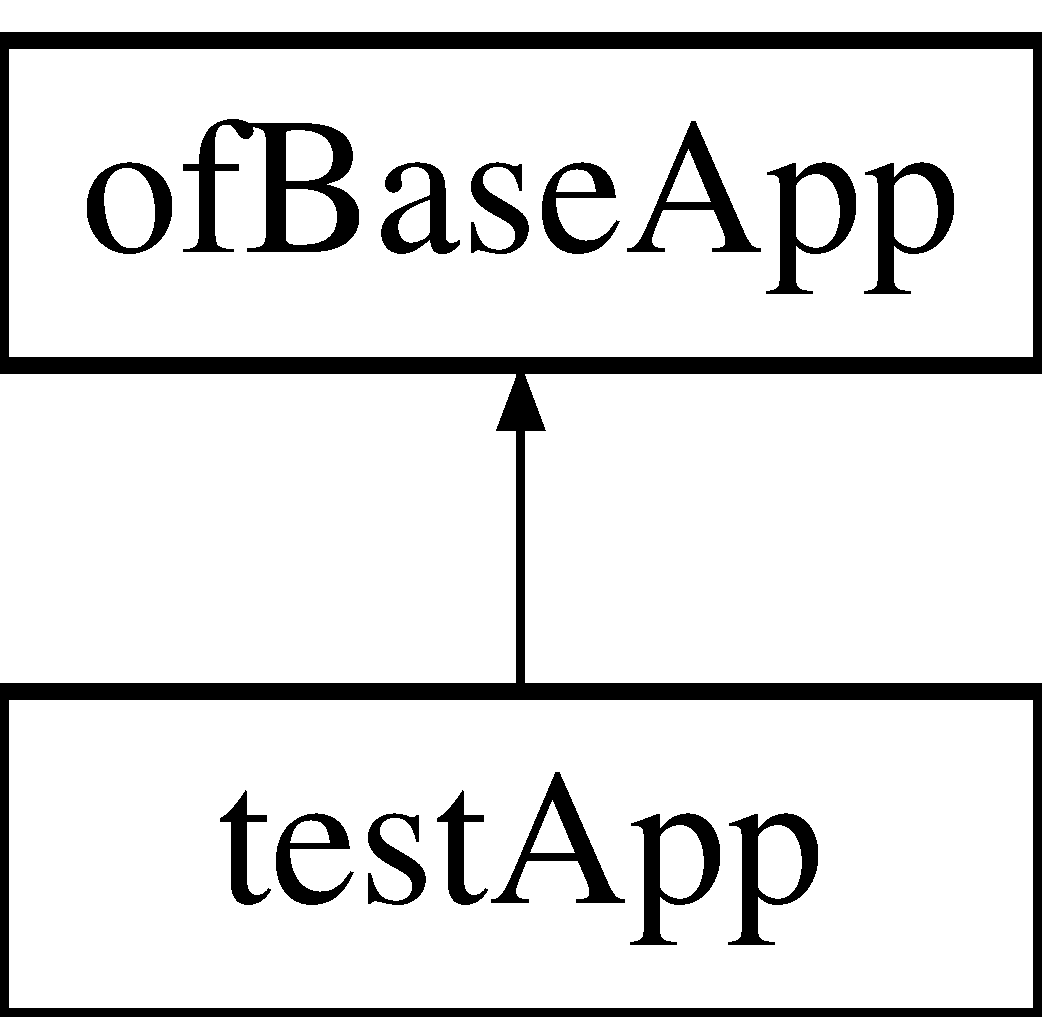
\includegraphics[height=2.000000cm]{classtest_app}
\end{center}
\end{figure}
\subsection*{Public Member Functions}
\begin{DoxyCompactItemize}
\item 
void \hyperlink{classtest_app_ad431db15b6150b965cd52bcba8e16e11}{setup} ()
\begin{DoxyCompactList}\small\item\em Setups this object. \end{DoxyCompactList}\item 
\hypertarget{classtest_app_afb39d201aec71a295b7609876bf7d0c6}{void {\bfseries update} ()}\label{classtest_app_afb39d201aec71a295b7609876bf7d0c6}

\item 
void \hyperlink{classtest_app_af869cba67b1dab8481f8d0e216d59dcd}{draw} ()
\item 
void \hyperlink{classtest_app_a904d147c7e532cb92656d5dd4895cd26}{key\-Pressed} (int key)
\item 
\hypertarget{classtest_app_a1116a10088e4932f6d482efe723cd45e}{void {\bfseries key\-Released} (int key)}\label{classtest_app_a1116a10088e4932f6d482efe723cd45e}

\item 
\hypertarget{classtest_app_a33541b19eff9f8285b2487bfc146d58b}{void {\bfseries mouse\-Moved} (int x, int y)}\label{classtest_app_a33541b19eff9f8285b2487bfc146d58b}

\item 
\hypertarget{classtest_app_a075bcc2be16fd8f3eaa9162fb40a0a1f}{void {\bfseries mouse\-Dragged} (int x, int y, int button)}\label{classtest_app_a075bcc2be16fd8f3eaa9162fb40a0a1f}

\item 
void \hyperlink{classtest_app_a3f200702ce91859cac2872a39302679d}{mouse\-Pressed} (int x, int y, int button)
\begin{DoxyCompactList}\small\item\em Mouse pressed. \end{DoxyCompactList}\item 
void \hyperlink{classtest_app_aa3680ffc782b1e5c451289817f20c9c6}{mouse\-Released} (int x, int y, int button)
\begin{DoxyCompactList}\small\item\em Mouse released. \end{DoxyCompactList}\item 
\hypertarget{classtest_app_a428b7df9c64352d6e7cb234fc297e6c9}{void {\bfseries window\-Resized} (int w, int h)}\label{classtest_app_a428b7df9c64352d6e7cb234fc297e6c9}

\item 
void \hyperlink{classtest_app_a853bbabdab3e7d2f207bb5a2028990bd}{Update\-Tracking} ()
\begin{DoxyCompactList}\small\item\em Updates the tracking. \end{DoxyCompactList}\item 
\hypertarget{classtest_app_a6a4db7a6a914fc4899763fc94bfca4b7}{void {\bfseries setup\-Tracker} ()}\label{classtest_app_a6a4db7a6a914fc4899763fc94bfca4b7}

\item 
void \hyperlink{classtest_app_af88f7715b2e0a9692b4ec947fad63c31}{setup\-Models} ()
\item 
void \hyperlink{classtest_app_a78bdea262a12308cb6f9f9243bdb3db9}{draw\-Models} ()
\item 
void \hyperlink{group___int_variables_gaa2fcbae31171ba366d4c0fcaf44149f4}{draw\-Axes} ()
\item 
void \hyperlink{group___int_variables_ga47747729f6d0d84c36ef0ec9fca01303}{draw\-Plane} ()
\begin{DoxyCompactList}\small\item\em Draw plane. \end{DoxyCompactList}\item 
void \hyperlink{group___int_variables_gae18e12d5025a2167ebd63ca019468cc0}{U\-D\-P\-Receive} ()
\item 
void \hyperlink{group___int_variables_gaa1d58aa9130d8d7526eb407f13f7a833}{add\-Objectto\-Scene} (string)
\item 
\hypertarget{group___int_variables_ga689f3b0cf0b38217152da7f5ce0d609f}{of\-Color {\bfseries Returncolor} (string)}\label{group___int_variables_ga689f3b0cf0b38217152da7f5ce0d609f}

\item 
void \hyperlink{group___int_variables_ga34646de458b0af33bc02457c9b8583df}{draw\-Augmented\-Plane} (float, float, of\-Color, of\-Color, int, string, string)
\begin{DoxyCompactList}\small\item\em Draw augmented plane. \end{DoxyCompactList}\item 
void \hyperlink{group___int_variables_ga16036c3aa23c1747e315a3e18105cf45}{draw\-Touches} (string udp\-Message)
\begin{DoxyCompactList}\small\item\em If the Handheld is being used a controller,This function will take the touch information and draw it on the A\-R view. \end{DoxyCompactList}\end{DoxyCompactItemize}
\subsection*{Public Attributes}
\begin{DoxyCompactItemize}
\item 
\hypertarget{classtest_app_a30c39505591fda7ed8ef4d8c4f0128fd}{ofx\-U\-D\-P\-Manager \hyperlink{classtest_app_a30c39505591fda7ed8ef4d8c4f0128fd}{udp\-Connection}}\label{classtest_app_a30c39505591fda7ed8ef4d8c4f0128fd}

\begin{DoxyCompactList}\small\item\em The U\-D\-P connection. \end{DoxyCompactList}\item 
\hypertarget{classtest_app_a35f96e427475843d44539f125ca454cd}{ofx\-U\-D\-P\-Manager \hyperlink{classtest_app_a35f96e427475843d44539f125ca454cd}{udp\-Send\-Connection}}\label{classtest_app_a35f96e427475843d44539f125ca454cd}

\begin{DoxyCompactList}\small\item\em The U\-D\-P send connection. \end{DoxyCompactList}\item 
\hypertarget{classtest_app_a630d5b8b53aee0c07dc79db616f4eb48}{ofx\-U\-D\-P\-Manager \hyperlink{classtest_app_a630d5b8b53aee0c07dc79db616f4eb48}{udp\-Receive\-Connection}}\label{classtest_app_a630d5b8b53aee0c07dc79db616f4eb48}

\begin{DoxyCompactList}\small\item\em The U\-D\-P receive connection. \end{DoxyCompactList}\item 
\hypertarget{classtest_app_a9bcefa3afb830941451f72174a36b722}{of\-True\-Type\-Font \hyperlink{classtest_app_a9bcefa3afb830941451f72174a36b722}{mono}}\label{classtest_app_a9bcefa3afb830941451f72174a36b722}

\begin{DoxyCompactList}\small\item\em The mono. \end{DoxyCompactList}\item 
\hypertarget{classtest_app_afc42ad25d37b1292d27d783380249424}{of\-True\-Type\-Font \hyperlink{classtest_app_afc42ad25d37b1292d27d783380249424}{monosm}}\label{classtest_app_afc42ad25d37b1292d27d783380249424}

\begin{DoxyCompactList}\small\item\em The monosm. \end{DoxyCompactList}\item 
\hypertarget{group___int_variables_ga9ed611377cd46f5148a3a3d538e96484}{int {\bfseries window\-Width}}\label{group___int_variables_ga9ed611377cd46f5148a3a3d538e96484}

\item 
int \hyperlink{group___int_variables_ga31efaa85f8a900bb659a537d56c73e03}{window\-Height}
\begin{DoxyCompactList}\small\item\em Gets the height of the window. \end{DoxyCompactList}\end{DoxyCompactItemize}
\begin{Indent}{\bf The Assimp\-Model\-Loader Variables ..}\par
{\em Black\-Bay \hyperlink{class_models}{Models} ..

These Variables will load all the \hyperlink{class_models}{Models} that were used for the Black\-Bay\-A\-R demo . }\begin{DoxyCompactItemize}
\item 
\hypertarget{group___int_variables_ga55051db1203331adb5556373b1f93194}{ofx\-Assimp\-Model\-Loader {\bfseries bb\-\_\-model}}\label{group___int_variables_ga55051db1203331adb5556373b1f93194}

\item 
\hypertarget{group___int_variables_ga0226f29cac900da4a7d1a698b1b5b9d3}{ofx\-Assimp\-Model\-Loader {\bfseries cr\-\_\-model}}\label{group___int_variables_ga0226f29cac900da4a7d1a698b1b5b9d3}

\item 
\hypertarget{group___int_variables_ga75d1f2c61d9e27b0f639a2632de94ed0}{ofx\-Assimp\-Model\-Loader {\bfseries lr\-\_\-model}}\label{group___int_variables_ga75d1f2c61d9e27b0f639a2632de94ed0}

\item 
\hypertarget{group___int_variables_gab7fc48fde55ff01601e7ec704685fda7}{ofx\-Assimp\-Model\-Loader {\bfseries ls\-\_\-model}}\label{group___int_variables_gab7fc48fde55ff01601e7ec704685fda7}

\item 
\hypertarget{group___int_variables_ga80f171a105bccdb3e505d438462d089a}{ofx\-Assimp\-Model\-Loader {\bfseries pgn\-\_\-model}}\label{group___int_variables_ga80f171a105bccdb3e505d438462d089a}

\item 
\hypertarget{group___int_variables_gaf98c6967c563936d418bf048a7d392b7}{ofx\-Assimp\-Model\-Loader {\bfseries pgy\-\_\-model}}\label{group___int_variables_gaf98c6967c563936d418bf048a7d392b7}

\item 
\hypertarget{group___int_variables_ga28a2622b1304d4096d4fefc1a46759b3}{ofx\-Assimp\-Model\-Loader {\bfseries pog\-\_\-model}}\label{group___int_variables_ga28a2622b1304d4096d4fefc1a46759b3}

\item 
\hypertarget{group___int_variables_ga24711bff00befce43455ad79653d388d}{ofx\-Assimp\-Model\-Loader {\bfseries rc\-\_\-model}}\label{group___int_variables_ga24711bff00befce43455ad79653d388d}

\item 
\hypertarget{group___int_variables_ga74279f23511603111eb4126414556b1b}{ofx\-Assimp\-Model\-Loader {\bfseries sr\-\_\-model}}\label{group___int_variables_ga74279f23511603111eb4126414556b1b}

\item 
\hypertarget{group___int_variables_ga56819e740669b8f1b443bdee23851442}{ofx\-Assimp\-Model\-Loader {\bfseries tbox\-\_\-model}}\label{group___int_variables_ga56819e740669b8f1b443bdee23851442}

\item 
\hypertarget{group___int_variables_ga6319a81becbadfcdd229bf2c98a7f930}{ofx\-Assimp\-Model\-Loader {\bfseries squirrel\-Model}}\label{group___int_variables_ga6319a81becbadfcdd229bf2c98a7f930}

\end{DoxyCompactItemize}
\end{Indent}


\subsection{Detailed Description}
Test application. 

\begin{DoxyAuthor}{Author}
Rahul 
\end{DoxyAuthor}
\begin{DoxyDate}{Date}
9/21/2012 
\end{DoxyDate}


\subsection{Member Function Documentation}
\hypertarget{classtest_app_af869cba67b1dab8481f8d0e216d59dcd}{\index{test\-App@{test\-App}!draw@{draw}}
\index{draw@{draw}!testApp@{test\-App}}
\subsubsection[{draw}]{\setlength{\rightskip}{0pt plus 5cm}void test\-App\-::draw (
\begin{DoxyParamCaption}
{}
\end{DoxyParamCaption}
)}}\label{classtest_app_af869cba67b1dab8481f8d0e216d59dcd}
Constructor.

\begin{DoxyAuthor}{Author}
Rahul 
\end{DoxyAuthor}
\begin{DoxyDate}{Date}
9/21/2012
\end{DoxyDate}

\begin{DoxyParams}{Parameters}
{\em parameter1} & The first parameter.\\
\hline
\end{DoxyParams}
\hypertarget{classtest_app_a78bdea262a12308cb6f9f9243bdb3db9}{\index{test\-App@{test\-App}!draw\-Models@{draw\-Models}}
\index{draw\-Models@{draw\-Models}!testApp@{test\-App}}
\subsubsection[{draw\-Models}]{\setlength{\rightskip}{0pt plus 5cm}void test\-App\-::draw\-Models (
\begin{DoxyParamCaption}
{}
\end{DoxyParamCaption}
)}}\label{classtest_app_a78bdea262a12308cb6f9f9243bdb3db9}
Constructor.

\begin{DoxyAuthor}{Author}
Rahul 
\end{DoxyAuthor}
\begin{DoxyDate}{Date}
9/21/2012
\end{DoxyDate}

\begin{DoxyParams}{Parameters}
{\em parameter1} & The first parameter. \\
\hline
{\em parameter2} & The second parameter.\\
\hline
\end{DoxyParams}
\hypertarget{classtest_app_a904d147c7e532cb92656d5dd4895cd26}{\index{test\-App@{test\-App}!key\-Pressed@{key\-Pressed}}
\index{key\-Pressed@{key\-Pressed}!testApp@{test\-App}}
\subsubsection[{key\-Pressed}]{\setlength{\rightskip}{0pt plus 5cm}void test\-App\-::key\-Pressed (
\begin{DoxyParamCaption}
\item[{int}]{key}
\end{DoxyParamCaption}
)}}\label{classtest_app_a904d147c7e532cb92656d5dd4895cd26}
Key released.

\begin{DoxyAuthor}{Author}
Rahul 
\end{DoxyAuthor}
\begin{DoxyDate}{Date}
9/21/2012
\end{DoxyDate}

\begin{DoxyParams}{Parameters}
{\em key} & The key.\\
\hline
\end{DoxyParams}
\hypertarget{classtest_app_a3f200702ce91859cac2872a39302679d}{\index{test\-App@{test\-App}!mouse\-Pressed@{mouse\-Pressed}}
\index{mouse\-Pressed@{mouse\-Pressed}!testApp@{test\-App}}
\subsubsection[{mouse\-Pressed}]{\setlength{\rightskip}{0pt plus 5cm}void test\-App\-::mouse\-Pressed (
\begin{DoxyParamCaption}
\item[{int}]{x, }
\item[{int}]{y, }
\item[{int}]{button}
\end{DoxyParamCaption}
)}}\label{classtest_app_a3f200702ce91859cac2872a39302679d}


Mouse pressed. 

This function will be called when the mouse is pressed

\begin{DoxyAuthor}{Author}
Rahul 
\end{DoxyAuthor}
\begin{DoxyDate}{Date}
9/21/2012
\end{DoxyDate}

\begin{DoxyParams}{Parameters}
{\em x} & The x coordinate. \\
\hline
{\em y} & The y coordinate. \\
\hline
{\em button} & The button. \\
\hline
\end{DoxyParams}
\hypertarget{classtest_app_aa3680ffc782b1e5c451289817f20c9c6}{\index{test\-App@{test\-App}!mouse\-Released@{mouse\-Released}}
\index{mouse\-Released@{mouse\-Released}!testApp@{test\-App}}
\subsubsection[{mouse\-Released}]{\setlength{\rightskip}{0pt plus 5cm}void test\-App\-::mouse\-Released (
\begin{DoxyParamCaption}
\item[{int}]{x, }
\item[{int}]{y, }
\item[{int}]{button}
\end{DoxyParamCaption}
)}}\label{classtest_app_aa3680ffc782b1e5c451289817f20c9c6}


Mouse released. 

\begin{DoxyAuthor}{Author}
Rahul 
\end{DoxyAuthor}
\begin{DoxyDate}{Date}
9/21/2012
\end{DoxyDate}

\begin{DoxyParams}{Parameters}
{\em x} & The x coordinate. \\
\hline
{\em y} & The y coordinate. \\
\hline
{\em button} & The button. \\
\hline
\end{DoxyParams}
\hypertarget{classtest_app_ad431db15b6150b965cd52bcba8e16e11}{\index{test\-App@{test\-App}!setup@{setup}}
\index{setup@{setup}!testApp@{test\-App}}
\subsubsection[{setup}]{\setlength{\rightskip}{0pt plus 5cm}void test\-App\-::setup (
\begin{DoxyParamCaption}
{}
\end{DoxyParamCaption}
)}}\label{classtest_app_ad431db15b6150b965cd52bcba8e16e11}


Setups this object. 

\begin{DoxyAuthor}{Author}
Rahul 
\end{DoxyAuthor}
\begin{DoxyDate}{Date}
9/21/2012 
\end{DoxyDate}
Constructor.

\begin{DoxyAuthor}{Author}
Rahul 
\end{DoxyAuthor}
\begin{DoxyDate}{Date}
9/21/2012
\end{DoxyDate}

\begin{DoxyParams}{Parameters}
{\em parameter1} & The first parameter.\\
\hline
\end{DoxyParams}
\hypertarget{classtest_app_af88f7715b2e0a9692b4ec947fad63c31}{\index{test\-App@{test\-App}!setup\-Models@{setup\-Models}}
\index{setup\-Models@{setup\-Models}!testApp@{test\-App}}
\subsubsection[{setup\-Models}]{\setlength{\rightskip}{0pt plus 5cm}void test\-App\-::setup\-Models (
\begin{DoxyParamCaption}
{}
\end{DoxyParamCaption}
)}}\label{classtest_app_af88f7715b2e0a9692b4ec947fad63c31}
Constructor.

\begin{DoxyAuthor}{Author}
Rahul 
\end{DoxyAuthor}
\begin{DoxyDate}{Date}
9/21/2012
\end{DoxyDate}

\begin{DoxyParams}{Parameters}
{\em parameter1} & The first parameter. \\
\hline
{\em parameter2} & The second parameter. \\
\hline
{\em parameter3} & The third parameter.\\
\hline
\end{DoxyParams}
\hypertarget{classtest_app_a853bbabdab3e7d2f207bb5a2028990bd}{\index{test\-App@{test\-App}!Update\-Tracking@{Update\-Tracking}}
\index{Update\-Tracking@{Update\-Tracking}!testApp@{test\-App}}
\subsubsection[{Update\-Tracking}]{\setlength{\rightskip}{0pt plus 5cm}void test\-App\-::\-Update\-Tracking (
\begin{DoxyParamCaption}
{}
\end{DoxyParamCaption}
)}}\label{classtest_app_a853bbabdab3e7d2f207bb5a2028990bd}


Updates the tracking. 

\begin{DoxyAuthor}{Author}
Rahul 
\end{DoxyAuthor}
\begin{DoxyDate}{Date}
9/21/2012 
\end{DoxyDate}


The documentation for this class was generated from the following files\-:\begin{DoxyCompactItemize}
\item 
src/\hyperlink{test_app_8h}{test\-App.\-h}\item 
src/\hyperlink{test_app_8cpp}{test\-App.\-cpp}\end{DoxyCompactItemize}

\chapter{File Documentation}
\hypertarget{test_app_8cpp}{\section{src/test\-App.cpp File Reference}
\label{test_app_8cpp}\index{src/test\-App.\-cpp@{src/test\-App.\-cpp}}
}


Implements the test application class.  


{\ttfamily \#include \char`\"{}test\-App.\-h\char`\"{}}\\*
{\ttfamily \#include \char`\"{}stdafx.\-h\char`\"{}}\\*
{\ttfamily \#include \char`\"{}I\-W\-Rsdk.\-h\char`\"{}}\\*
{\ttfamily \#include $<$stdio.\-h$>$}\\*
{\ttfamily \#include $<$fcntl.\-h$>$}\\*
{\ttfamily \#include $<$io.\-h$>$}\\*
{\ttfamily \#include $<$sys\textbackslash{}stat.\-h$>$}\\*
{\ttfamily \#include $<$iostream$>$}\\*
\subsection*{Namespaces}
\begin{DoxyCompactItemize}
\item 
namespace \hyperlink{namespacestd}{std}
\begin{DoxyCompactList}\small\item\em \end{DoxyCompactList}\end{DoxyCompactItemize}
\subsection*{Macros}
\begin{DoxyCompactItemize}
\item 
\#define \hyperlink{test_app_8cpp_af3fff26dd0daf747313fea22d007e08f}{I\-W\-R\-\_\-\-O\-K}~0
\begin{DoxyCompactList}\small\item\em A macro that defines iwr ok. \end{DoxyCompactList}\item 
\hypertarget{test_app_8cpp_a2700b1789448312031a74498f20c6151}{\#define {\bfseries I\-W\-R\-\_\-\-N\-O\-\_\-\-T\-R\-A\-C\-K\-E\-R}~1}\label{test_app_8cpp_a2700b1789448312031a74498f20c6151}

\item 
\#define \hyperlink{test_app_8cpp_a76171800ff5c2c8a68158b633bf34224}{I\-W\-R\-\_\-\-O\-F\-F\-L\-I\-N\-E}~2
\begin{DoxyCompactList}\small\item\em A macro that defines iwr offline. \end{DoxyCompactList}\item 
\hypertarget{test_app_8cpp_a396a3b6ee3905182e93a223c5baba939}{\#define {\bfseries I\-W\-R\-\_\-\-T\-R\-A\-C\-K\-E\-R\-\_\-\-C\-O\-R\-R\-U\-P\-T}~3}\label{test_app_8cpp_a396a3b6ee3905182e93a223c5baba939}

\item 
\#define \hyperlink{test_app_8cpp_a0133f9ab2073f3ed92ed68ab31207461}{I\-W\-R\-\_\-\-N\-O\-T\-R\-A\-C\-K\-E\-R\-\_\-\-I\-N\-S\-T\-A\-N\-C\-E}~4
\begin{DoxyCompactList}\small\item\em A macro that defines iwr notracker instance. \end{DoxyCompactList}\item 
\hypertarget{test_app_8cpp_a6ac55ca9ec2b159b660ad85684feffa7}{\#define {\bfseries I\-W\-R\-\_\-\-N\-O\-\_\-\-S\-T\-E\-R\-E\-O}~5}\label{test_app_8cpp_a6ac55ca9ec2b159b660ad85684feffa7}

\item 
\#define \hyperlink{test_app_8cpp_abf7f3ce37211489caedaaecd77232c35}{I\-W\-R\-\_\-\-S\-T\-E\-R\-E\-O\-\_\-\-C\-O\-R\-R\-U\-P\-T}~6
\begin{DoxyCompactList}\small\item\em A macro that defines iwr stereo corrupt. \end{DoxyCompactList}\end{DoxyCompactItemize}
\subsection*{Enumerations}
\begin{DoxyCompactItemize}
\item 
enum \{ {\bfseries N\-O\-\_\-\-F\-I\-L\-T\-E\-R} =0, 
{\bfseries A\-P\-P\-L\-I\-C\-A\-T\-I\-O\-N\-\_\-\-F\-I\-L\-T\-E\-R}, 
{\bfseries I\-N\-T\-E\-R\-N\-A\-L\-\_\-\-F\-I\-L\-T\-E\-R}
 \}
\end{DoxyCompactItemize}
\subsection*{Functions}
\begin{DoxyCompactItemize}
\item 
\hypertarget{test_app_8cpp_abc3d99fdd08f8cf5968947ade2874ec5}{void {\bfseries I\-W\-R\-Filter\-Tracking} (long $\ast$\hyperlink{test_app_8cpp_a7efc219781df4a1e281cb5d348b7fbf9}{yaw}, long $\ast$pitch, long $\ast$roll)}\label{test_app_8cpp_abc3d99fdd08f8cf5968947ade2874ec5}

\end{DoxyCompactItemize}
\subsection*{Variables}
\begin{DoxyCompactItemize}
\item 
\hypertarget{test_app_8cpp_a176d63bc2538f9abe94a1a39f88348ed}{bool {\bfseries g\-\_\-tracking} = false}\label{test_app_8cpp_a176d63bc2538f9abe94a1a39f88348ed}

\item 
\hypertarget{test_app_8cpp_a5b7b2353e37b213f7d54fd5c41405e6d}{float \hyperlink{test_app_8cpp_a5b7b2353e37b213f7d54fd5c41405e6d}{g\-\_\-f\-Yaw} = 0.\-0f}\label{test_app_8cpp_a5b7b2353e37b213f7d54fd5c41405e6d}

\begin{DoxyCompactList}\small\item\em The roll. \end{DoxyCompactList}\item 
\hypertarget{test_app_8cpp_a03b98db700342d558e183b7f610f957e}{float {\bfseries g\-\_\-f\-Pitch} = 0.\-0f}\label{test_app_8cpp_a03b98db700342d558e183b7f610f957e}

\item 
\hypertarget{test_app_8cpp_a4c06be914a849a84a818cfb2a8f192a8}{float {\bfseries g\-\_\-f\-Roll} = 0.\-0f}\label{test_app_8cpp_a4c06be914a849a84a818cfb2a8f192a8}

\item 
\hypertarget{test_app_8cpp_a20de1ec8e34993508aef934f2ea06149}{long \hyperlink{test_app_8cpp_a20de1ec8e34993508aef934f2ea06149}{iwr\-\_\-status}}\label{test_app_8cpp_a20de1ec8e34993508aef934f2ea06149}

\begin{DoxyCompactList}\small\item\em The iwr status. \end{DoxyCompactList}\item 
\hypertarget{test_app_8cpp_a3a1437b324a10893d0a616cd086c6271}{int \hyperlink{test_app_8cpp_a3a1437b324a10893d0a616cd086c6271}{g\-\_\-\-Filtering} = 0}\label{test_app_8cpp_a3a1437b324a10893d0a616cd086c6271}

\begin{DoxyCompactList}\small\item\em The filtering. \end{DoxyCompactList}\item 
\hypertarget{test_app_8cpp_a0868f931f3e011d04c6a7072fd91a576}{int \hyperlink{test_app_8cpp_a0868f931f3e011d04c6a7072fd91a576}{Pid} = 0}\label{test_app_8cpp_a0868f931f3e011d04c6a7072fd91a576}

\begin{DoxyCompactList}\small\item\em The P\-I\-D. \end{DoxyCompactList}\item 
\hypertarget{test_app_8cpp_a639c84ce78fef8ba2780de9c25770791}{H\-M\-O\-D\-U\-L\-E {\bfseries h\-Mod}}\label{test_app_8cpp_a639c84ce78fef8ba2780de9c25770791}

\item 
\hypertarget{test_app_8cpp_a6a757ca08fc9a3db5efe516c2055fff7}{of\-Camera {\bfseries cam}}\label{test_app_8cpp_a6a757ca08fc9a3db5efe516c2055fff7}

\item 
float \hyperlink{test_app_8cpp_a7efc219781df4a1e281cb5d348b7fbf9}{yaw} =0
\begin{DoxyCompactList}\small\item\em -- Processing ... \end{DoxyCompactList}\item 
\hypertarget{test_app_8cpp_a26fd84d522945b6038221d9e38c7cc39}{float {\bfseries roll} =0}\label{test_app_8cpp_a26fd84d522945b6038221d9e38c7cc39}

\item 
\hypertarget{test_app_8cpp_a2a45ec4ebd7ddda05fdd49eb42148544}{vector$<$ \hyperlink{class_p_o_is}{P\-O\-Is} $>$ \hyperlink{test_app_8cpp_a2a45ec4ebd7ddda05fdd49eb42148544}{scenes}}\label{test_app_8cpp_a2a45ec4ebd7ddda05fdd49eb42148544}

\begin{DoxyCompactList}\small\item\em The scenes. \end{DoxyCompactList}\item 
\hypertarget{test_app_8cpp_ac440c8cafae97a89976b9bc5a60e90de}{vector$<$ \hyperlink{class_note_information}{Note\-Information} $>$ {\bfseries Notes}}\label{test_app_8cpp_ac440c8cafae97a89976b9bc5a60e90de}

\item 
\hypertarget{test_app_8cpp_ac9bfcbe432b145792a0b6a0eea4906c5}{float {\bfseries rot\-X}}\label{test_app_8cpp_ac9bfcbe432b145792a0b6a0eea4906c5}

\item 
float \hyperlink{test_app_8cpp_a677393b11ed5136b379e1b2d9ba008f1}{rot\-Y}
\begin{DoxyCompactList}\small\item\em Gets the rot y coordinate. \end{DoxyCompactList}\item 
\hypertarget{test_app_8cpp_acff4256798c08cf5ac9f0b6d961671be}{float \hyperlink{test_app_8cpp_acff4256798c08cf5ac9f0b6d961671be}{rot\-Angle} =0}\label{test_app_8cpp_acff4256798c08cf5ac9f0b6d961671be}

\begin{DoxyCompactList}\small\item\em The rot angle. \end{DoxyCompactList}\item 
\hypertarget{test_app_8cpp_a67edb40b2aec44dc1f59cc8ce5f4eb44}{of\-Image \hyperlink{test_app_8cpp_a67edb40b2aec44dc1f59cc8ce5f4eb44}{crosshair}}\label{test_app_8cpp_a67edb40b2aec44dc1f59cc8ce5f4eb44}

\begin{DoxyCompactList}\small\item\em The crosshair. \end{DoxyCompactList}\item 
\hypertarget{test_app_8cpp_afef2218c3159c33bb3e2a84280541309}{float \hyperlink{test_app_8cpp_afef2218c3159c33bb3e2a84280541309}{initialyaw} =0}\label{test_app_8cpp_afef2218c3159c33bb3e2a84280541309}

\begin{DoxyCompactList}\small\item\em The initialyaw. \end{DoxyCompactList}\item 
\hypertarget{test_app_8cpp_acb559820d9ca11295b4500f179ef6392}{int \hyperlink{test_app_8cpp_acb559820d9ca11295b4500f179ef6392}{i}}\label{test_app_8cpp_acb559820d9ca11295b4500f179ef6392}

\begin{DoxyCompactList}\small\item\em Zero-\/based index of the. \end{DoxyCompactList}\item 
\hypertarget{test_app_8cpp_ab1b4d9fb9f738cef6f815a498af72064}{\hyperlink{class_calculations}{Calculations} {\bfseries calc}}\label{test_app_8cpp_ab1b4d9fb9f738cef6f815a498af72064}

\item 
\hypertarget{test_app_8cpp_ac95cac19f6a7a7db0e4a6347af105547}{vector$<$ string $>$ \hyperlink{test_app_8cpp_ac95cac19f6a7a7db0e4a6347af105547}{result}}\label{test_app_8cpp_ac95cac19f6a7a7db0e4a6347af105547}

\begin{DoxyCompactList}\small\item\em \end{DoxyCompactList}\item 
\hypertarget{test_app_8cpp_a32c6734ce7abc3300b2239785b23df5c}{of\-Color \hyperlink{test_app_8cpp_a32c6734ce7abc3300b2239785b23df5c}{white} =of\-Color\-::from\-Hex(0xffffff)}\label{test_app_8cpp_a32c6734ce7abc3300b2239785b23df5c}

\begin{DoxyCompactList}\small\item\em The white. \end{DoxyCompactList}\item 
\hypertarget{test_app_8cpp_aa58af911ab57bdf37823dcd2286e4c66}{of\-Color {\bfseries green} = of\-Color\-::from\-Hex(0x00ff00)}\label{test_app_8cpp_aa58af911ab57bdf37823dcd2286e4c66}

\item 
\hypertarget{test_app_8cpp_a2d0305516339ed5db19b9a2f8e8869e8}{of\-Color \hyperlink{test_app_8cpp_a2d0305516339ed5db19b9a2f8e8869e8}{blue} =of\-Color\-::from\-Hex(0x0000ff)}\label{test_app_8cpp_a2d0305516339ed5db19b9a2f8e8869e8}

\begin{DoxyCompactList}\small\item\em The blue. \end{DoxyCompactList}\item 
\hypertarget{test_app_8cpp_af306de37383449d0273c65e01df28bcf}{of\-Color {\bfseries yellow} =of\-Color\-::from\-Hex(0xffff00)}\label{test_app_8cpp_af306de37383449d0273c65e01df28bcf}

\item 
\hypertarget{test_app_8cpp_a69aedf2df8226da8bdbb25f31c6aae51}{of\-Color \hyperlink{test_app_8cpp_a69aedf2df8226da8bdbb25f31c6aae51}{red} =of\-Color\-::from\-Hex(0xff0000)}\label{test_app_8cpp_a69aedf2df8226da8bdbb25f31c6aae51}

\begin{DoxyCompactList}\small\item\em The red. \end{DoxyCompactList}\item 
\hypertarget{test_app_8cpp_adda20be792fdf00d6ed4a0ef65883e51}{of\-Color {\bfseries black} =of\-Color\-::from\-Hex(0x000000)}\label{test_app_8cpp_adda20be792fdf00d6ed4a0ef65883e51}

\item 
\hypertarget{test_app_8cpp_aa6f56bb80388eba91f06c92632bc1dda}{of\-True\-Type\-Font \hyperlink{test_app_8cpp_aa6f56bb80388eba91f06c92632bc1dda}{Serif\-\_\-15}}\label{test_app_8cpp_aa6f56bb80388eba91f06c92632bc1dda}

\begin{DoxyCompactList}\small\item\em The fifth serif 1. \end{DoxyCompactList}\item 
\hypertarget{test_app_8cpp_ac1daf15866a617ff20285b658d2e6ce4}{of\-True\-Type\-Font {\bfseries Serif\-\_\-10}}\label{test_app_8cpp_ac1daf15866a617ff20285b658d2e6ce4}

\end{DoxyCompactItemize}


\subsection{Detailed Description}
Implements the test application class. 

\subsection{Macro Definition Documentation}
\hypertarget{test_app_8cpp_a0133f9ab2073f3ed92ed68ab31207461}{\index{test\-App.\-cpp@{test\-App.\-cpp}!I\-W\-R\-\_\-\-N\-O\-T\-R\-A\-C\-K\-E\-R\-\_\-\-I\-N\-S\-T\-A\-N\-C\-E@{I\-W\-R\-\_\-\-N\-O\-T\-R\-A\-C\-K\-E\-R\-\_\-\-I\-N\-S\-T\-A\-N\-C\-E}}
\index{I\-W\-R\-\_\-\-N\-O\-T\-R\-A\-C\-K\-E\-R\-\_\-\-I\-N\-S\-T\-A\-N\-C\-E@{I\-W\-R\-\_\-\-N\-O\-T\-R\-A\-C\-K\-E\-R\-\_\-\-I\-N\-S\-T\-A\-N\-C\-E}!testApp.cpp@{test\-App.\-cpp}}
\subsubsection[{I\-W\-R\-\_\-\-N\-O\-T\-R\-A\-C\-K\-E\-R\-\_\-\-I\-N\-S\-T\-A\-N\-C\-E}]{\setlength{\rightskip}{0pt plus 5cm}\#define I\-W\-R\-\_\-\-N\-O\-T\-R\-A\-C\-K\-E\-R\-\_\-\-I\-N\-S\-T\-A\-N\-C\-E~4}}\label{test_app_8cpp_a0133f9ab2073f3ed92ed68ab31207461}


A macro that defines iwr notracker instance. 

\begin{DoxyAuthor}{Author}
Rahul 
\end{DoxyAuthor}
\begin{DoxyDate}{Date}
9/21/2012 
\end{DoxyDate}
\hypertarget{test_app_8cpp_a76171800ff5c2c8a68158b633bf34224}{\index{test\-App.\-cpp@{test\-App.\-cpp}!I\-W\-R\-\_\-\-O\-F\-F\-L\-I\-N\-E@{I\-W\-R\-\_\-\-O\-F\-F\-L\-I\-N\-E}}
\index{I\-W\-R\-\_\-\-O\-F\-F\-L\-I\-N\-E@{I\-W\-R\-\_\-\-O\-F\-F\-L\-I\-N\-E}!testApp.cpp@{test\-App.\-cpp}}
\subsubsection[{I\-W\-R\-\_\-\-O\-F\-F\-L\-I\-N\-E}]{\setlength{\rightskip}{0pt plus 5cm}\#define I\-W\-R\-\_\-\-O\-F\-F\-L\-I\-N\-E~2}}\label{test_app_8cpp_a76171800ff5c2c8a68158b633bf34224}


A macro that defines iwr offline. 

\begin{DoxyAuthor}{Author}
Rahul 
\end{DoxyAuthor}
\begin{DoxyDate}{Date}
9/21/2012 
\end{DoxyDate}
\hypertarget{test_app_8cpp_af3fff26dd0daf747313fea22d007e08f}{\index{test\-App.\-cpp@{test\-App.\-cpp}!I\-W\-R\-\_\-\-O\-K@{I\-W\-R\-\_\-\-O\-K}}
\index{I\-W\-R\-\_\-\-O\-K@{I\-W\-R\-\_\-\-O\-K}!testApp.cpp@{test\-App.\-cpp}}
\subsubsection[{I\-W\-R\-\_\-\-O\-K}]{\setlength{\rightskip}{0pt plus 5cm}\#define I\-W\-R\-\_\-\-O\-K~0}}\label{test_app_8cpp_af3fff26dd0daf747313fea22d007e08f}


A macro that defines iwr ok. 

\begin{DoxyAuthor}{Author}
Rahul 
\end{DoxyAuthor}
\begin{DoxyDate}{Date}
9/21/2012 
\end{DoxyDate}
\hypertarget{test_app_8cpp_abf7f3ce37211489caedaaecd77232c35}{\index{test\-App.\-cpp@{test\-App.\-cpp}!I\-W\-R\-\_\-\-S\-T\-E\-R\-E\-O\-\_\-\-C\-O\-R\-R\-U\-P\-T@{I\-W\-R\-\_\-\-S\-T\-E\-R\-E\-O\-\_\-\-C\-O\-R\-R\-U\-P\-T}}
\index{I\-W\-R\-\_\-\-S\-T\-E\-R\-E\-O\-\_\-\-C\-O\-R\-R\-U\-P\-T@{I\-W\-R\-\_\-\-S\-T\-E\-R\-E\-O\-\_\-\-C\-O\-R\-R\-U\-P\-T}!testApp.cpp@{test\-App.\-cpp}}
\subsubsection[{I\-W\-R\-\_\-\-S\-T\-E\-R\-E\-O\-\_\-\-C\-O\-R\-R\-U\-P\-T}]{\setlength{\rightskip}{0pt plus 5cm}\#define I\-W\-R\-\_\-\-S\-T\-E\-R\-E\-O\-\_\-\-C\-O\-R\-R\-U\-P\-T~6}}\label{test_app_8cpp_abf7f3ce37211489caedaaecd77232c35}


A macro that defines iwr stereo corrupt. 

\begin{DoxyAuthor}{Author}
Rahul 
\end{DoxyAuthor}
\begin{DoxyDate}{Date}
9/21/2012 
\end{DoxyDate}


\subsection{Variable Documentation}
\hypertarget{test_app_8cpp_a677393b11ed5136b379e1b2d9ba008f1}{\index{test\-App.\-cpp@{test\-App.\-cpp}!rot\-Y@{rot\-Y}}
\index{rot\-Y@{rot\-Y}!testApp.cpp@{test\-App.\-cpp}}
\subsubsection[{rot\-Y}]{\setlength{\rightskip}{0pt plus 5cm}float rot\-X rot\-Y}}\label{test_app_8cpp_a677393b11ed5136b379e1b2d9ba008f1}


Gets the rot y coordinate. 

\begin{DoxyReturn}{Returns}
The rot y coordinate. 
\end{DoxyReturn}
\hypertarget{test_app_8cpp_a7efc219781df4a1e281cb5d348b7fbf9}{\index{test\-App.\-cpp@{test\-App.\-cpp}!yaw@{yaw}}
\index{yaw@{yaw}!testApp.cpp@{test\-App.\-cpp}}
\subsubsection[{yaw}]{\setlength{\rightskip}{0pt plus 5cm}float yaw =0}}\label{test_app_8cpp_a7efc219781df4a1e281cb5d348b7fbf9}


-- Processing ... 

The roll. 
\hypertarget{test_app_8h}{\section{src/test\-App.h File Reference}
\label{test_app_8h}\index{src/test\-App.\-h@{src/test\-App.\-h}}
}


Declares the test application class.  


{\ttfamily \#include \char`\"{}of\-Main.\-h\char`\"{}}\\*
{\ttfamily \#include \char`\"{}ofx\-Network.\-h\char`\"{}}\\*
{\ttfamily \#include \char`\"{}of\-Vec3f.\-h\char`\"{}}\\*
{\ttfamily \#include \char`\"{}ofx\-Assimp\-Model\-Loader.\-h\char`\"{}}\\*
{\ttfamily \#include \char`\"{}of\-Camera.\-h\char`\"{}}\\*
{\ttfamily \#include \char`\"{}Calculations.\-h\char`\"{}}\\*
{\ttfamily \#include \char`\"{}Note\-Information.\-h\char`\"{}}\\*
{\ttfamily \#include \char`\"{}ofx\-Xml\-Settings.\-h\char`\"{}}\\*
{\ttfamily \#include $<$list$>$}\\*
{\ttfamily \#include $<$Models.\-h$>$}\\*
\subsection*{Classes}
\begin{DoxyCompactItemize}
\item 
class \hyperlink{classtest_app}{test\-App}
\begin{DoxyCompactList}\small\item\em Test application. \end{DoxyCompactList}\end{DoxyCompactItemize}


\subsection{Detailed Description}
Declares the test application class. 
\addcontentsline{toc}{part}{Index}
\printindex
\end{document}
